\documentclass[twoside]{book}

% Packages required by doxygen
\usepackage{fixltx2e}
\usepackage{calc}
\usepackage{doxygen}
\usepackage[export]{adjustbox} % also loads graphicx
\usepackage{graphicx}
\usepackage[utf8]{inputenc}
\usepackage{makeidx}
\usepackage{multicol}
\usepackage{multirow}
\PassOptionsToPackage{warn}{textcomp}
\usepackage{textcomp}
\usepackage[nointegrals]{wasysym}
\usepackage[table]{xcolor}

% NLS support packages
\usepackage[spanish]{babel}
% Font selection
\usepackage[T1]{fontenc}
\usepackage[scaled=.90]{helvet}
\usepackage{courier}
\usepackage{amssymb}
\usepackage{sectsty}
\renewcommand{\familydefault}{\sfdefault}
\allsectionsfont{%
  \fontseries{bc}\selectfont%
  \color{darkgray}%
}
\renewcommand{\DoxyLabelFont}{%
  \fontseries{bc}\selectfont%
  \color{darkgray}%
}
\newcommand{\+}{\discretionary{\mbox{\scriptsize$\hookleftarrow$}}{}{}}

% Page & text layout
\usepackage{geometry}
\geometry{%
  a4paper,%
  top=2.5cm,%
  bottom=2.5cm,%
  left=2.5cm,%
  right=2.5cm%
}
\tolerance=750
\hfuzz=15pt
\hbadness=750
\setlength{\emergencystretch}{15pt}
\setlength{\parindent}{0cm}
\setlength{\parskip}{3ex plus 2ex minus 2ex}
\makeatletter
\renewcommand{\paragraph}{%
  \@startsection{paragraph}{4}{0ex}{-1.0ex}{1.0ex}{%
    \normalfont\normalsize\bfseries\SS@parafont%
  }%
}
\renewcommand{\subparagraph}{%
  \@startsection{subparagraph}{5}{0ex}{-1.0ex}{1.0ex}{%
    \normalfont\normalsize\bfseries\SS@subparafont%
  }%
}
\makeatother

% Headers & footers
\usepackage{fancyhdr}
\pagestyle{fancyplain}
\fancyhead[LE]{\fancyplain{}{\bfseries\thepage}}
\fancyhead[CE]{\fancyplain{}{}}
\fancyhead[RE]{\fancyplain{}{\bfseries\leftmark}}
\fancyhead[LO]{\fancyplain{}{\bfseries\rightmark}}
\fancyhead[CO]{\fancyplain{}{}}
\fancyhead[RO]{\fancyplain{}{\bfseries\thepage}}
\fancyfoot[LE]{\fancyplain{}{}}
\fancyfoot[CE]{\fancyplain{}{}}
\fancyfoot[RE]{\fancyplain{}{\bfseries\scriptsize Generado por Doxygen }}
\fancyfoot[LO]{\fancyplain{}{\bfseries\scriptsize Generado por Doxygen }}
\fancyfoot[CO]{\fancyplain{}{}}
\fancyfoot[RO]{\fancyplain{}{}}
\renewcommand{\footrulewidth}{0.4pt}
\renewcommand{\chaptermark}[1]{%
  \markboth{#1}{}%
}
\renewcommand{\sectionmark}[1]{%
  \markright{\thesection\ #1}%
}

% Indices & bibliography
\usepackage{natbib}
\usepackage[titles]{tocloft}
\setcounter{tocdepth}{3}
\setcounter{secnumdepth}{5}
\makeindex

% Hyperlinks (required, but should be loaded last)
\usepackage{ifpdf}
\ifpdf
  \usepackage[pdftex,pagebackref=true]{hyperref}
\else
  \usepackage[ps2pdf,pagebackref=true]{hyperref}
\fi
\hypersetup{%
  colorlinks=true,%
  linkcolor=blue,%
  citecolor=blue,%
  unicode%
}

% Custom commands
\newcommand{\clearemptydoublepage}{%
  \newpage{\pagestyle{empty}\cleardoublepage}%
}

\usepackage{caption}
\captionsetup{labelsep=space,justification=centering,font={bf},singlelinecheck=off,skip=4pt,position=top}

%===== C O N T E N T S =====

\begin{document}

% Titlepage & ToC
\hypersetup{pageanchor=false,
             bookmarksnumbered=true,
             pdfencoding=unicode
            }
\pagenumbering{alph}
\begin{titlepage}
\vspace*{7cm}
\begin{center}%
{\Large Laboratorio de P\+R\+O2. Gestion de un almacen \\[1ex]\large v5.\+0 26-\/05-\/2018 }\\
\vspace*{1cm}
{\large Generado por Doxygen 1.8.13}\\
\end{center}
\end{titlepage}
\clearemptydoublepage
\pagenumbering{roman}
\tableofcontents
\clearemptydoublepage
\pagenumbering{arabic}
\hypersetup{pageanchor=true}

%--- Begin generated contents ---
\chapter{Ejemplo de diseño modular\+: Gestión de un almacen.}
\label{index}\hypertarget{index}{}En esta practica se construye un programa modular que ofrece un menú de opciones para gestionar un almacen. Se introducen las clases {\itshape \hyperlink{class_cjt__productos}{Cjt\+\_\+productos}}, {\itshape \hyperlink{class_sala}{Sala}}, {\itshape \hyperlink{class_cjt__salas}{Cjt\+\_\+salas}} y {\itshape \hyperlink{class_almacen}{Almacen}}. 
\chapter{Índice de clases}
\section{Llista de Classes}
Aquestes són les classes, estructures, unions i interfícies acompanyades amb breus descripcions\+:\begin{DoxyCompactList}
\item\contentsline{section}{\hyperlink{class_cjt__estudiants}{Cjt\+\_\+estudiants} \\*Representa un conjunt d\textquotesingle{}estudiants ordenat per D\+NI }{\pageref{class_cjt__estudiants}}{}
\item\contentsline{section}{\hyperlink{class_estudiant}{Estudiant} \\*Representa un estudiant amb D\+NI i la possibilitat de tenir nota }{\pageref{class_estudiant}}{}
\end{DoxyCompactList}

\chapter{Indice de archivos}
\section{Llista dels Fitxers}
Aquesta és la llista de tots els fitxers acompanyats amb breus descripcions\+:\begin{DoxyCompactList}
\item\contentsline{section}{\hyperlink{_bin_tree_8hh}{Bin\+Tree.\+hh} }{\pageref{_bin_tree_8hh}}{}
\item\contentsline{section}{\hyperlink{_cjt___clusters_8cc}{Cjt\+\_\+\+Clusters.\+cc} \\*Implementació de la classe \hyperlink{class_cjt___clusters}{Cjt\+\_\+\+Clusters} }{\pageref{_cjt___clusters_8cc}}{}
\item\contentsline{section}{\hyperlink{_cjt___clusters_8hh}{Cjt\+\_\+\+Clusters.\+hh} \\*Especificació de la classe \hyperlink{class_cjt___clusters}{Cjt\+\_\+\+Clusters} }{\pageref{_cjt___clusters_8hh}}{}
\item\contentsline{section}{\hyperlink{_cjt___especies_8cc}{Cjt\+\_\+\+Especies.\+cc} \\*Implementació de la classe \hyperlink{class_cjt___especies}{Cjt\+\_\+\+Especies} }{\pageref{_cjt___especies_8cc}}{}
\item\contentsline{section}{\hyperlink{_cjt___especies_8hh}{Cjt\+\_\+\+Especies.\+hh} \\*Especificació de la classe \hyperlink{class_cjt___especies}{Cjt\+\_\+\+Especies} }{\pageref{_cjt___especies_8hh}}{}
\item\contentsline{section}{\hyperlink{_cluster_8cc}{Cluster.\+cc} \\*Implementació de la classe \hyperlink{class_cluster}{Cluster} }{\pageref{_cluster_8cc}}{}
\item\contentsline{section}{\hyperlink{_cluster_8hh}{Cluster.\+hh} \\*Especificació de la classe \hyperlink{class_cluster}{Cluster} }{\pageref{_cluster_8hh}}{}
\item\contentsline{section}{\hyperlink{_especie_8cc}{Especie.\+cc} \\*Implementació de la classe \hyperlink{class_especie}{Especie} }{\pageref{_especie_8cc}}{}
\item\contentsline{section}{\hyperlink{_especie_8hh}{Especie.\+hh} \\*Especificació de la classe \hyperlink{class_especie}{Especie} }{\pageref{_especie_8hh}}{}
\item\contentsline{section}{\hyperlink{program_8cc}{program.\+cc} \\*Programa principal de la pràctica }{\pageref{program_8cc}}{}
\end{DoxyCompactList}

\chapter{Documentación de las clases}
\hypertarget{class_almacen}{}\section{Referencia de la Clase Almacen}
\label{class_almacen}\index{Almacen@{Almacen}}


Representa la estructura del almacen.  


\subsection*{Métodos públicos}
\begin{DoxyCompactItemize}
\item 
\hyperlink{class_almacen_a68a6084d5775d391c52d4825072a0612}{Almacen} ()
\begin{DoxyCompactList}\small\item\em Creadora por defecto. \end{DoxyCompactList}\item 
\hyperlink{class_almacen_a1f4b6a1196d0c571c06012096e9401a2}{Almacen} (Bin\+Tree$<$ int $>$ aux)
\begin{DoxyCompactList}\small\item\em Copiadora por defecto. \end{DoxyCompactList}\item 
Bin\+Tree$<$ int $>$ \hyperlink{class_almacen_af16a0a319f91554aad713c14ee95715b}{consultar\+\_\+almacen} ()
\begin{DoxyCompactList}\small\item\em Consultora del almacen. \end{DoxyCompactList}\item 
\hyperlink{class_almacen}{Almacen} \hyperlink{class_almacen_a36e2c6293837248738e5783e8e69795d}{leer\+\_\+almacen} ()
\begin{DoxyCompactList}\small\item\em Se lee la distribucion de las salas del almacen. \end{DoxyCompactList}\item 
void \hyperlink{class_almacen_a0757bdd016511f5b2b1019060c0b2a9c}{escribir} ()
\begin{DoxyCompactList}\small\item\em Operación de escritura. \end{DoxyCompactList}\end{DoxyCompactItemize}
\subsection*{Atributos privados}
\begin{DoxyCompactItemize}
\item 
Bin\+Tree$<$ int $>$ \hyperlink{class_almacen_a0744bed3ca8c796990c939bbf7fc03b9}{estructura\+\_\+almacen}
\begin{DoxyCompactList}\small\item\em Arbol que representa la estructura del almacen. \end{DoxyCompactList}\end{DoxyCompactItemize}


\subsection{Descripción detallada}
Representa la estructura del almacen. 

Representa la estructura del almacen con un arbol en que cada nodo contiene el identificador de sala 

Definición en la línea 20 del archivo Almacen.\+hh.



\subsection{Documentación del constructor y destructor}
\mbox{\Hypertarget{class_almacen_a68a6084d5775d391c52d4825072a0612}\label{class_almacen_a68a6084d5775d391c52d4825072a0612}} 
\index{Almacen@{Almacen}!Almacen@{Almacen}}
\index{Almacen@{Almacen}!Almacen@{Almacen}}
\subsubsection{\texorpdfstring{Almacen()}{Almacen()}\hspace{0.1cm}{\footnotesize\ttfamily [1/2]}}
{\footnotesize\ttfamily Almacen\+::\+Almacen (\begin{DoxyParamCaption}{ }\end{DoxyParamCaption})}



Creadora por defecto. 

Se ejecuta automáticamente al declarar un almacen. \begin{DoxyPrecond}{Precondición}
{\itshape cierto} 
\end{DoxyPrecond}
\begin{DoxyPostcond}{Postcondición}
El resultado es un almacen 
\end{DoxyPostcond}


Definición en la línea 7 del archivo Almacen.\+cc.


\begin{DoxyCode}
8 \{ 
9 \}
\end{DoxyCode}
\mbox{\Hypertarget{class_almacen_a1f4b6a1196d0c571c06012096e9401a2}\label{class_almacen_a1f4b6a1196d0c571c06012096e9401a2}} 
\index{Almacen@{Almacen}!Almacen@{Almacen}}
\index{Almacen@{Almacen}!Almacen@{Almacen}}
\subsubsection{\texorpdfstring{Almacen()}{Almacen()}\hspace{0.1cm}{\footnotesize\ttfamily [2/2]}}
{\footnotesize\ttfamily Almacen\+::\+Almacen (\begin{DoxyParamCaption}\item[{Bin\+Tree$<$ int $>$}]{aux }\end{DoxyParamCaption})}



Copiadora por defecto. 

Se introduce un arbol y devuelve un almacen

\begin{DoxyPrecond}{Precondición}
{\itshape cierto} 
\end{DoxyPrecond}
\begin{DoxyPostcond}{Postcondición}
El resultado es un almacen 
\end{DoxyPostcond}


Definición en la línea 10 del archivo Almacen.\+cc.


\begin{DoxyCode}
11 \{
12   \hyperlink{class_almacen_a0744bed3ca8c796990c939bbf7fc03b9}{estructura\_almacen}=aux;
13  
14 \}
\end{DoxyCode}


\subsection{Documentación de las funciones miembro}
\mbox{\Hypertarget{class_almacen_af16a0a319f91554aad713c14ee95715b}\label{class_almacen_af16a0a319f91554aad713c14ee95715b}} 
\index{Almacen@{Almacen}!consultar\+\_\+almacen@{consultar\+\_\+almacen}}
\index{consultar\+\_\+almacen@{consultar\+\_\+almacen}!Almacen@{Almacen}}
\subsubsection{\texorpdfstring{consultar\+\_\+almacen()}{consultar\_almacen()}}
{\footnotesize\ttfamily Bin\+Tree$<$ int $>$ Almacen\+::consultar\+\_\+almacen (\begin{DoxyParamCaption}{ }\end{DoxyParamCaption})}



Consultora del almacen. 

Devuelve el arbol del parametro implcito estructura\+\_\+almacen

\begin{DoxyPrecond}{Precondición}
{\itshape cierto} 
\end{DoxyPrecond}
\begin{DoxyPostcond}{Postcondición}
El resultado es el arbol de la estructura del almacen 
\end{DoxyPostcond}


Definición en la línea 16 del archivo Almacen.\+cc.


\begin{DoxyCode}
16                                        \{
17     \textcolor{keywordflow}{return} \hyperlink{class_almacen_a0744bed3ca8c796990c939bbf7fc03b9}{estructura\_almacen}; \textcolor{comment}{// devuelve el p.i. del almacen}
18 \}
\end{DoxyCode}
\mbox{\Hypertarget{class_almacen_a36e2c6293837248738e5783e8e69795d}\label{class_almacen_a36e2c6293837248738e5783e8e69795d}} 
\index{Almacen@{Almacen}!leer\+\_\+almacen@{leer\+\_\+almacen}}
\index{leer\+\_\+almacen@{leer\+\_\+almacen}!Almacen@{Almacen}}
\subsubsection{\texorpdfstring{leer\+\_\+almacen()}{leer\_almacen()}}
{\footnotesize\ttfamily \hyperlink{class_almacen}{Almacen} Almacen\+::leer\+\_\+almacen (\begin{DoxyParamCaption}{ }\end{DoxyParamCaption})}



Se lee la distribucion de las salas del almacen. 

En el canal estandard hay una serie de enteros, si el entero es 0 significa que el arbol no continua por uno de los subarboles posibles \begin{DoxyPrecond}{Precondición}
En el canal estandard de entrada estan preparados una serie de enteros que representan la estructura del almacen 
\end{DoxyPrecond}
\begin{DoxyPostcond}{Postcondición}
El parámetro implícito contiene un arbol que representa la estructura del almacen teniendo en cuenta los parametros entrados 
\end{DoxyPostcond}


Definición en la línea 22 del archivo Almacen.\+cc.


\begin{DoxyCode}
23 \{   
24     \textcolor{keywordtype}{int} x;
25     cin>>x ;
26     \textcolor{keywordflow}{if}( x!=0)\{  \textcolor{comment}{//marca}
27         \hyperlink{class_almacen}{Almacen} e,d;
28         e=\hyperlink{class_almacen_a36e2c6293837248738e5783e8e69795d}{leer\_almacen}();
29         d=\hyperlink{class_almacen_a36e2c6293837248738e5783e8e69795d}{leer\_almacen}();
30         \hyperlink{class_almacen_a0744bed3ca8c796990c939bbf7fc03b9}{estructura\_almacen}= BinTree<int> (x, e.
      \hyperlink{class_almacen_af16a0a319f91554aad713c14ee95715b}{consultar\_almacen}(), d.\hyperlink{class_almacen_af16a0a319f91554aad713c14ee95715b}{consultar\_almacen}());
31     \}
32     \textcolor{keywordflow}{else} \textcolor{keywordflow}{return} \hyperlink{class_almacen_a68a6084d5775d391c52d4825072a0612}{Almacen}(); \textcolor{comment}{//devuelve un almacen vacio}
33     \textcolor{keywordflow}{return} \hyperlink{class_almacen_a68a6084d5775d391c52d4825072a0612}{Almacen}(\hyperlink{class_almacen_a0744bed3ca8c796990c939bbf7fc03b9}{estructura\_almacen});
34    
35 
36 \}
\end{DoxyCode}
\mbox{\Hypertarget{class_almacen_a0757bdd016511f5b2b1019060c0b2a9c}\label{class_almacen_a0757bdd016511f5b2b1019060c0b2a9c}} 
\index{Almacen@{Almacen}!escribir@{escribir}}
\index{escribir@{escribir}!Almacen@{Almacen}}
\subsubsection{\texorpdfstring{escribir()}{escribir()}}
{\footnotesize\ttfamily void Almacen\+::escribir (\begin{DoxyParamCaption}{ }\end{DoxyParamCaption})}



Operación de escritura. 

\begin{DoxyPrecond}{Precondición}
El parámetro implícito está inicializado 
\end{DoxyPrecond}
\begin{DoxyPostcond}{Postcondición}
Escribe las propiedades y el contenido del parámetro implícito por el canal estándar de salida 
\end{DoxyPostcond}


Definición en la línea 38 del archivo Almacen.\+cc.


\begin{DoxyCode}
39 \{   
40     cout<<\hyperlink{class_almacen_a0744bed3ca8c796990c939bbf7fc03b9}{estructura\_almacen}.value()<<\textcolor{stringliteral}{" "};
41     \hyperlink{class_almacen}{Almacen} a;
42     \textcolor{keywordflow}{if}(!\hyperlink{class_almacen_a0744bed3ca8c796990c939bbf7fc03b9}{estructura\_almacen}.left().empty())\{
43         a=\hyperlink{class_almacen_a68a6084d5775d391c52d4825072a0612}{Almacen}(\hyperlink{class_almacen_a0744bed3ca8c796990c939bbf7fc03b9}{estructura\_almacen}.left());
44         a.\hyperlink{class_almacen_a0757bdd016511f5b2b1019060c0b2a9c}{escribir}();
45     \}
46     \textcolor{keywordflow}{if}(!\hyperlink{class_almacen_a0744bed3ca8c796990c939bbf7fc03b9}{estructura\_almacen}.right().empty())\{
47         a=\hyperlink{class_almacen_a68a6084d5775d391c52d4825072a0612}{Almacen}(\hyperlink{class_almacen_a0744bed3ca8c796990c939bbf7fc03b9}{estructura\_almacen}.right());
48         a.\hyperlink{class_almacen_a0757bdd016511f5b2b1019060c0b2a9c}{escribir}();
49     \}
50 
51 \}
\end{DoxyCode}


\subsection{Documentación de los datos miembro}
\mbox{\Hypertarget{class_almacen_a0744bed3ca8c796990c939bbf7fc03b9}\label{class_almacen_a0744bed3ca8c796990c939bbf7fc03b9}} 
\index{Almacen@{Almacen}!estructura\+\_\+almacen@{estructura\+\_\+almacen}}
\index{estructura\+\_\+almacen@{estructura\+\_\+almacen}!Almacen@{Almacen}}
\subsubsection{\texorpdfstring{estructura\+\_\+almacen}{estructura\_almacen}}
{\footnotesize\ttfamily Bin\+Tree$<$int$>$ Almacen\+::estructura\+\_\+almacen\hspace{0.3cm}{\ttfamily [private]}}



Arbol que representa la estructura del almacen. 



Definición en la línea 75 del archivo Almacen.\+hh.



La documentación para esta clase fue generada a partir de los siguientes ficheros\+:\begin{DoxyCompactItemize}
\item 
\hyperlink{_almacen_8hh}{Almacen.\+hh}\item 
\hyperlink{_almacen_8cc}{Almacen.\+cc}\end{DoxyCompactItemize}

\hypertarget{class_cjt__productos}{}\section{Referencia de la Clase Cjt\+\_\+productos}
\label{class_cjt__productos}\index{Cjt\+\_\+productos@{Cjt\+\_\+productos}}


Representa el inventario del almacen con atributos identificador y unidades.  


\subsection*{Métodos públicos}
\begin{DoxyCompactItemize}
\item 
void \hyperlink{class_cjt__productos_a501153e137c6437ff84faac121a88bc8}{poner\+\_\+prod} (string iden\+\_\+prod)
\begin{DoxyCompactList}\small\item\em Modificadora con valores concretos. \end{DoxyCompactList}\item 
void \hyperlink{class_cjt__productos_a2da6626c288772c1169dcf32c39202e6}{quitar\+\_\+prod} (string iden\+\_\+prod)
\begin{DoxyCompactList}\small\item\em Destructora con valores concretos. \end{DoxyCompactList}\item 
void \hyperlink{class_cjt__productos_ac120487a0d46654b0d89654f20055083}{modificar} (string iden\+\_\+prod, int uni\+\_\+prod)
\begin{DoxyCompactList}\small\item\em Modificadora de los atributos. \end{DoxyCompactList}\item 
int \hyperlink{class_cjt__productos_a8198f3b57f6d1d9fd4096e3e19fe9a46}{consultar\+\_\+prod} (string iden\+\_\+prod)
\begin{DoxyCompactList}\small\item\em Consultora de las unidades. \end{DoxyCompactList}\item 
bool \hyperlink{class_cjt__productos_a33f8148c4da6fe03d49c993e4b477494}{existe\+\_\+prod} (string iden\+\_\+prod)
\begin{DoxyCompactList}\small\item\em Consultora de producto. \end{DoxyCompactList}\item 
void \hyperlink{class_cjt__productos_a51582783f3f107f84cc3c5f8cccded36}{escribir} ()
\begin{DoxyCompactList}\small\item\em Operación de escritura. \end{DoxyCompactList}\end{DoxyCompactItemize}
\subsection*{Atributos privados}
\begin{DoxyCompactItemize}
\item 
map$<$ string, int $>$ \hyperlink{class_cjt__productos_a44e63c644fdec6cff81dcdb3cf79860c}{map\+\_\+productos}
\begin{DoxyCompactList}\small\item\em inventario del almacen \end{DoxyCompactList}\item 
map$<$ string, int $>$\+::iterator \hyperlink{class_cjt__productos_adedbe2194ed053eb446ec367e6d5e60e}{it}
\begin{DoxyCompactList}\small\item\em iterador del inventario del almacen \end{DoxyCompactList}\end{DoxyCompactItemize}


\subsection{Descripción detallada}
Representa el inventario del almacen con atributos identificador y unidades. 

Definición en la línea 20 del archivo Cjt\+\_\+productos.\+hh.



\subsection{Documentación de las funciones miembro}
\mbox{\Hypertarget{class_cjt__productos_a501153e137c6437ff84faac121a88bc8}\label{class_cjt__productos_a501153e137c6437ff84faac121a88bc8}} 
\index{Cjt\+\_\+productos@{Cjt\+\_\+productos}!poner\+\_\+prod@{poner\+\_\+prod}}
\index{poner\+\_\+prod@{poner\+\_\+prod}!Cjt\+\_\+productos@{Cjt\+\_\+productos}}
\subsubsection{\texorpdfstring{poner\+\_\+prod()}{poner\_prod()}}
{\footnotesize\ttfamily void Cjt\+\_\+productos\+::poner\+\_\+prod (\begin{DoxyParamCaption}\item[{string}]{iden\+\_\+prod }\end{DoxyParamCaption})}



Modificadora con valores concretos. 

Se introduce un identificador de producto. Si el producto ya existia se produce un error, sino el producto se da de alta en el sistema con cero unidades. \begin{DoxyPrecond}{Precondición}
iden\+\_\+prod$>$0 
\end{DoxyPrecond}
\begin{DoxyPostcond}{Postcondición}
El resultado es una prenda con identificador \char`\"{}iden\+\_\+prod\char`\"{} y unidades \char`\"{}uni\+\_\+prod\char`\"{} 0 
\end{DoxyPostcond}


Definición en la línea 7 del archivo Cjt\+\_\+productos.\+cc.


\begin{DoxyCode}
8 \{
9   \textcolor{keywordflow}{if}(iden\_prod>\textcolor{stringliteral}{""})\{
10     \hyperlink{class_cjt__productos_adedbe2194ed053eb446ec367e6d5e60e}{it}=\hyperlink{class_cjt__productos_a44e63c644fdec6cff81dcdb3cf79860c}{map\_productos}.find(iden\_prod);
11     \textcolor{keywordflow}{if}(\hyperlink{class_cjt__productos_adedbe2194ed053eb446ec367e6d5e60e}{it}==\hyperlink{class_cjt__productos_a44e63c644fdec6cff81dcdb3cf79860c}{map\_productos}.end())\{
12       \hyperlink{class_cjt__productos_a44e63c644fdec6cff81dcdb3cf79860c}{map\_productos}[iden\_prod]=0; \textcolor{comment}{//pone producto con 0 unidades}
13     \}
14     \textcolor{keywordflow}{else} cout<<\textcolor{stringliteral}{"  error"}<<endl;
15   \}
16   \textcolor{keywordflow}{else}  cout<<\textcolor{stringliteral}{"  error"}<<endl;
17   
18 \}
\end{DoxyCode}
\mbox{\Hypertarget{class_cjt__productos_a2da6626c288772c1169dcf32c39202e6}\label{class_cjt__productos_a2da6626c288772c1169dcf32c39202e6}} 
\index{Cjt\+\_\+productos@{Cjt\+\_\+productos}!quitar\+\_\+prod@{quitar\+\_\+prod}}
\index{quitar\+\_\+prod@{quitar\+\_\+prod}!Cjt\+\_\+productos@{Cjt\+\_\+productos}}
\subsubsection{\texorpdfstring{quitar\+\_\+prod()}{quitar\_prod()}}
{\footnotesize\ttfamily void Cjt\+\_\+productos\+::quitar\+\_\+prod (\begin{DoxyParamCaption}\item[{string}]{iden\+\_\+prod }\end{DoxyParamCaption})}



Destructora con valores concretos. 

Se introduce un identificador de producto. Si el producto no existe, o ya existe y quedan unidades se produce un error, sino el producto se da de baja en el sistema. \begin{DoxyPrecond}{Precondición}
iden\+\_\+prod $>$0 
\end{DoxyPrecond}
\begin{DoxyPostcond}{Postcondición}
El resultado es que el producto se da de baja del sistema 
\end{DoxyPostcond}


Definición en la línea 20 del archivo Cjt\+\_\+productos.\+cc.


\begin{DoxyCode}
21 \{
22   \textcolor{keywordflow}{if}(iden\_prod>\textcolor{stringliteral}{""})\{
23     \hyperlink{class_cjt__productos_adedbe2194ed053eb446ec367e6d5e60e}{it}=\hyperlink{class_cjt__productos_a44e63c644fdec6cff81dcdb3cf79860c}{map\_productos}.find(iden\_prod);
24 
25     \textcolor{keywordflow}{if}(\hyperlink{class_cjt__productos_adedbe2194ed053eb446ec367e6d5e60e}{it}!=\hyperlink{class_cjt__productos_a44e63c644fdec6cff81dcdb3cf79860c}{map\_productos}.end())\{
26 
27       \textcolor{keywordflow}{if}(\hyperlink{class_cjt__productos_adedbe2194ed053eb446ec367e6d5e60e}{it}->second==0)\{
28 
29         \hyperlink{class_cjt__productos_a44e63c644fdec6cff81dcdb3cf79860c}{map\_productos}.erase(iden\_prod); \textcolor{comment}{//elimina si tiene 0 unidades}
30       \}
31       \textcolor{keywordflow}{else} cout<<\textcolor{stringliteral}{"  error"}<<endl;
32     \}
33     \textcolor{keywordflow}{else} cout<<\textcolor{stringliteral}{"  error"}<<endl;
34   \}
35   \textcolor{keywordflow}{else}  cout<<\textcolor{stringliteral}{"  error"}<<endl;
36 
37 \}
\end{DoxyCode}
\mbox{\Hypertarget{class_cjt__productos_ac120487a0d46654b0d89654f20055083}\label{class_cjt__productos_ac120487a0d46654b0d89654f20055083}} 
\index{Cjt\+\_\+productos@{Cjt\+\_\+productos}!modificar@{modificar}}
\index{modificar@{modificar}!Cjt\+\_\+productos@{Cjt\+\_\+productos}}
\subsubsection{\texorpdfstring{modificar()}{modificar()}}
{\footnotesize\ttfamily void Cjt\+\_\+productos\+::modificar (\begin{DoxyParamCaption}\item[{string}]{iden\+\_\+prod,  }\item[{int}]{uni\+\_\+prod }\end{DoxyParamCaption})}



Modificadora de los atributos. 

Se introduce un identificador de producto y sus unidades. Si el producto no existe o sus unidades son negativas da error. Sino el parametro implicito del producto con \char`\"{}iden\+\_\+prod\char`\"{} pasa a tener \char`\"{}uni\+\_\+prod\char`\"{} unidades \begin{DoxyPrecond}{Precondición}
iden\+\_\+prod$>$0 uni\+\_\+prod$>$=0 
\end{DoxyPrecond}
\begin{DoxyPostcond}{Postcondición}
El parámetro implícito pasa a tener identificador \char`\"{}iden\+\_\+prod\char`\"{}y unidades \char`\"{}uni\+\_\+prod\char`\"{} 
\end{DoxyPostcond}


Definición en la línea 39 del archivo Cjt\+\_\+productos.\+cc.


\begin{DoxyCode}
40 \{
41   \textcolor{keywordflow}{if}(iden\_prod>\textcolor{stringliteral}{""} and uni\_prod>=0)\{
42     \hyperlink{class_cjt__productos_adedbe2194ed053eb446ec367e6d5e60e}{it}=\hyperlink{class_cjt__productos_a44e63c644fdec6cff81dcdb3cf79860c}{map\_productos}.find(iden\_prod);
43     \textcolor{keywordflow}{if}(\hyperlink{class_cjt__productos_adedbe2194ed053eb446ec367e6d5e60e}{it}!=\hyperlink{class_cjt__productos_a44e63c644fdec6cff81dcdb3cf79860c}{map\_productos}.end())\{
44       \hyperlink{class_cjt__productos_adedbe2194ed053eb446ec367e6d5e60e}{it}->second= uni\_prod; 
45     \}
46     \textcolor{keywordflow}{else} cout<<\textcolor{stringliteral}{"  error"}<<endl;
47   \}
48   \textcolor{keywordflow}{else} cout<<\textcolor{stringliteral}{"  error"}<<endl;
49 \}
\end{DoxyCode}
\mbox{\Hypertarget{class_cjt__productos_a8198f3b57f6d1d9fd4096e3e19fe9a46}\label{class_cjt__productos_a8198f3b57f6d1d9fd4096e3e19fe9a46}} 
\index{Cjt\+\_\+productos@{Cjt\+\_\+productos}!consultar\+\_\+prod@{consultar\+\_\+prod}}
\index{consultar\+\_\+prod@{consultar\+\_\+prod}!Cjt\+\_\+productos@{Cjt\+\_\+productos}}
\subsubsection{\texorpdfstring{consultar\+\_\+prod()}{consultar\_prod()}}
{\footnotesize\ttfamily int Cjt\+\_\+productos\+::consultar\+\_\+prod (\begin{DoxyParamCaption}\item[{string}]{iden\+\_\+prod }\end{DoxyParamCaption})}



Consultora de las unidades. 

Se introduce un identificador de producto. Si no existe, se produce un error. Si existe se escribe cuantas unidades hay en total en el almacen. \begin{DoxyPrecond}{Precondición}
{\itshape cierto} 
\end{DoxyPrecond}
\begin{DoxyPostcond}{Postcondición}
El resultado son las unidades del parámetro implícito 
\end{DoxyPostcond}


Definición en la línea 51 del archivo Cjt\+\_\+productos.\+cc.


\begin{DoxyCode}
52 \{
53   \textcolor{keywordflow}{if}(iden\_prod>\textcolor{stringliteral}{""} )\{
54     \hyperlink{class_cjt__productos_adedbe2194ed053eb446ec367e6d5e60e}{it}=\hyperlink{class_cjt__productos_a44e63c644fdec6cff81dcdb3cf79860c}{map\_productos}.find(iden\_prod);
55     \textcolor{keywordflow}{if}(\hyperlink{class_cjt__productos_adedbe2194ed053eb446ec367e6d5e60e}{it}!=\hyperlink{class_cjt__productos_a44e63c644fdec6cff81dcdb3cf79860c}{map\_productos}.end())\{
56       \textcolor{keywordflow}{return}  \hyperlink{class_cjt__productos_adedbe2194ed053eb446ec367e6d5e60e}{it}->second;
57     \}
58     \textcolor{keywordflow}{else} cout<<\textcolor{stringliteral}{"  error"}<<endl;
59   \}
60   \textcolor{keywordflow}{else} cout<<\textcolor{stringliteral}{"  error"}<<endl;
61   \textcolor{keywordflow}{return} -1;
62 \}
\end{DoxyCode}
\mbox{\Hypertarget{class_cjt__productos_a33f8148c4da6fe03d49c993e4b477494}\label{class_cjt__productos_a33f8148c4da6fe03d49c993e4b477494}} 
\index{Cjt\+\_\+productos@{Cjt\+\_\+productos}!existe\+\_\+prod@{existe\+\_\+prod}}
\index{existe\+\_\+prod@{existe\+\_\+prod}!Cjt\+\_\+productos@{Cjt\+\_\+productos}}
\subsubsection{\texorpdfstring{existe\+\_\+prod()}{existe\_prod()}}
{\footnotesize\ttfamily bool Cjt\+\_\+productos\+::existe\+\_\+prod (\begin{DoxyParamCaption}\item[{string}]{iden\+\_\+prod }\end{DoxyParamCaption})}



Consultora de producto. 

Se introduce un identificador de producto. Si no existe devuelve falso. Si existe devuelve true. \begin{DoxyPrecond}{Precondición}
{\itshape cierto} 
\end{DoxyPrecond}
\begin{DoxyPostcond}{Postcondición}
El resultado es un booleano 
\end{DoxyPostcond}


Definición en la línea 64 del archivo Cjt\+\_\+productos.\+cc.


\begin{DoxyCode}
65 \{
66   \hyperlink{class_cjt__productos_adedbe2194ed053eb446ec367e6d5e60e}{it}=\hyperlink{class_cjt__productos_a44e63c644fdec6cff81dcdb3cf79860c}{map\_productos}.find(iden\_prod);
67   \textcolor{keywordflow}{if}(\hyperlink{class_cjt__productos_adedbe2194ed053eb446ec367e6d5e60e}{it}!=\hyperlink{class_cjt__productos_a44e63c644fdec6cff81dcdb3cf79860c}{map\_productos}.end())\{
68     \textcolor{keywordflow}{return}  \textcolor{keyword}{true};
69   \}
70   \textcolor{keywordflow}{else} \textcolor{keywordflow}{return} \textcolor{keyword}{false}; 
71 \}
\end{DoxyCode}
\mbox{\Hypertarget{class_cjt__productos_a51582783f3f107f84cc3c5f8cccded36}\label{class_cjt__productos_a51582783f3f107f84cc3c5f8cccded36}} 
\index{Cjt\+\_\+productos@{Cjt\+\_\+productos}!escribir@{escribir}}
\index{escribir@{escribir}!Cjt\+\_\+productos@{Cjt\+\_\+productos}}
\subsubsection{\texorpdfstring{escribir()}{escribir()}}
{\footnotesize\ttfamily void Cjt\+\_\+productos\+::escribir (\begin{DoxyParamCaption}{ }\end{DoxyParamCaption})}



Operación de escritura. 

Escribe por pantalla el inventario del almacen \begin{DoxyPrecond}{Precondición}
{\itshape cierto} 
\end{DoxyPrecond}
\begin{DoxyPostcond}{Postcondición}
Se han escrito los identificadores de producto que hay las estanterias. 
\end{DoxyPostcond}


Definición en la línea 73 del archivo Cjt\+\_\+productos.\+cc.


\begin{DoxyCode}
74 \{
75   \hyperlink{class_cjt__productos_adedbe2194ed053eb446ec367e6d5e60e}{it} = \hyperlink{class_cjt__productos_a44e63c644fdec6cff81dcdb3cf79860c}{map\_productos}.begin();
76   \textcolor{keywordflow}{while}(\hyperlink{class_cjt__productos_adedbe2194ed053eb446ec367e6d5e60e}{it}!=\hyperlink{class_cjt__productos_a44e63c644fdec6cff81dcdb3cf79860c}{map\_productos}.end())\{
77     cout<<\textcolor{stringliteral}{"  "}<<\hyperlink{class_cjt__productos_adedbe2194ed053eb446ec367e6d5e60e}{it}->first<<\textcolor{stringliteral}{" "}<<\hyperlink{class_cjt__productos_adedbe2194ed053eb446ec367e6d5e60e}{it}->second<<endl;
78     \hyperlink{class_cjt__productos_adedbe2194ed053eb446ec367e6d5e60e}{it}++;
79  \}
80 \}
\end{DoxyCode}


\subsection{Documentación de los datos miembro}
\mbox{\Hypertarget{class_cjt__productos_a44e63c644fdec6cff81dcdb3cf79860c}\label{class_cjt__productos_a44e63c644fdec6cff81dcdb3cf79860c}} 
\index{Cjt\+\_\+productos@{Cjt\+\_\+productos}!map\+\_\+productos@{map\+\_\+productos}}
\index{map\+\_\+productos@{map\+\_\+productos}!Cjt\+\_\+productos@{Cjt\+\_\+productos}}
\subsubsection{\texorpdfstring{map\+\_\+productos}{map\_productos}}
{\footnotesize\ttfamily map$<$string, int$>$ Cjt\+\_\+productos\+::map\+\_\+productos\hspace{0.3cm}{\ttfamily [private]}}



inventario del almacen 



Definición en la línea 95 del archivo Cjt\+\_\+productos.\+hh.

\mbox{\Hypertarget{class_cjt__productos_adedbe2194ed053eb446ec367e6d5e60e}\label{class_cjt__productos_adedbe2194ed053eb446ec367e6d5e60e}} 
\index{Cjt\+\_\+productos@{Cjt\+\_\+productos}!it@{it}}
\index{it@{it}!Cjt\+\_\+productos@{Cjt\+\_\+productos}}
\subsubsection{\texorpdfstring{it}{it}}
{\footnotesize\ttfamily map$<$string,int$>$\+::iterator Cjt\+\_\+productos\+::it\hspace{0.3cm}{\ttfamily [private]}}



iterador del inventario del almacen 



Definición en la línea 97 del archivo Cjt\+\_\+productos.\+hh.



La documentación para esta clase fue generada a partir de los siguientes ficheros\+:\begin{DoxyCompactItemize}
\item 
\hyperlink{_cjt__productos_8hh}{Cjt\+\_\+productos.\+hh}\item 
\hyperlink{_cjt__productos_8cc}{Cjt\+\_\+productos.\+cc}\end{DoxyCompactItemize}

\hypertarget{class_cjt__salas}{}\section{Referencia de la Clase Cjt\+\_\+salas}
\label{class_cjt__salas}\index{Cjt\+\_\+salas@{Cjt\+\_\+salas}}


Representa un conjunto de salas.  


\subsection*{Métodos públicos}
\begin{DoxyCompactItemize}
\item 
int \hyperlink{class_cjt__salas_ab9f5c933dbf2fa1c0bedf0ff5ae6eeb8}{poner\+\_\+items} (int iden\+\_\+sala, string iden\+\_\+prod, int uni\+\_\+prod)
\begin{DoxyCompactList}\small\item\em Añade varias unidades de un producto a la sala. \end{DoxyCompactList}\item 
int \hyperlink{class_cjt__salas_acd5d8368e51d7bbd557958063c81cc43}{quitar\+\_\+items} (int iden\+\_\+sala, string iden\+\_\+prod, int uni\+\_\+prod)
\begin{DoxyCompactList}\small\item\em Quita varios productos de la sala. \end{DoxyCompactList}\item 
void \hyperlink{class_cjt__salas_a1ecd0e8e0ae84290c354447e2a305e80}{compactar} (int iden\+\_\+sala)
\begin{DoxyCompactList}\small\item\em Compacta una estanteria. \end{DoxyCompactList}\item 
void \hyperlink{class_cjt__salas_a540d49e9ee9a7a078e18f610399335b6}{reorganizar} (int iden\+\_\+sala)
\begin{DoxyCompactList}\small\item\em Reorganiza una estanteria. \end{DoxyCompactList}\item 
void \hyperlink{class_cjt__salas_af4a9c609def322edba117ae76aa0b3b9}{redimensionar} (int iden\+\_\+sala, int filas, int columnas)
\begin{DoxyCompactList}\small\item\em Compacta una estanteria. \end{DoxyCompactList}\item 
string \hyperlink{class_cjt__salas_a7e06b122fbbee58f24b8938bc2975b16}{consultar\+\_\+pos} (int iden\+\_\+sala, int filas, int columnas)
\begin{DoxyCompactList}\small\item\em Consultora de un producto. \end{DoxyCompactList}\item 
void \hyperlink{class_cjt__salas_ae79acb3461bd487e7bda3af42a3f96b7}{leer} (int num\+\_\+sala)
\begin{DoxyCompactList}\small\item\em Operación de escritura. \end{DoxyCompactList}\item 
void \hyperlink{class_cjt__salas_a184f3ef5d7857c7f76ecef58b093f252}{escribir} (int iden\+\_\+sala)
\begin{DoxyCompactList}\small\item\em Operación de escritura. \end{DoxyCompactList}\end{DoxyCompactItemize}
\subsection*{Atributos privados}
\begin{DoxyCompactItemize}
\item 
vector$<$ \hyperlink{class_sala}{Sala} $>$ \hyperlink{class_cjt__salas_a3f130cc8bab35f449de8be69283af09e}{vec\+\_\+salas}
\begin{DoxyCompactList}\small\item\em Vector que representa el conjunto de salas del almacen. \end{DoxyCompactList}\end{DoxyCompactItemize}


\subsection{Descripción detallada}
Representa un conjunto de salas. 

Puede contener las diferentes salas de un almacen con las caracteristicas de cada sala 

Definición en la línea 20 del archivo Cjt\+\_\+salas.\+hh.



\subsection{Documentación de las funciones miembro}
\mbox{\Hypertarget{class_cjt__salas_ab9f5c933dbf2fa1c0bedf0ff5ae6eeb8}\label{class_cjt__salas_ab9f5c933dbf2fa1c0bedf0ff5ae6eeb8}} 
\index{Cjt\+\_\+salas@{Cjt\+\_\+salas}!poner\+\_\+items@{poner\+\_\+items}}
\index{poner\+\_\+items@{poner\+\_\+items}!Cjt\+\_\+salas@{Cjt\+\_\+salas}}
\subsubsection{\texorpdfstring{poner\+\_\+items()}{poner\_items()}}
{\footnotesize\ttfamily int Cjt\+\_\+salas\+::poner\+\_\+items (\begin{DoxyParamCaption}\item[{int}]{iden\+\_\+sala,  }\item[{string}]{iden\+\_\+prod,  }\item[{int}]{uni\+\_\+prod }\end{DoxyParamCaption})}



Añade varias unidades de un producto a la sala. 

Se introduce un identificador de sala, un identificador de producto y una cantidad. Si el producto no existe se produce un error. Se colocan tantas unidades como quepan en la sala y se devuelve un entero que indique cuantas unidades no han cabido. Se colocaran las unidades lo antes posible, es decir, primero se rellenan los huecos a partir del hueco que vaya antes. Las unidades que no quepan no se guardan en el almacen. \begin{DoxyPrecond}{Precondición}
1$<$=iden\+\_\+sala$<$=n iden\+\_\+prod$>$0 uni\+\_\+prod$>$0 
\end{DoxyPrecond}
\begin{DoxyPostcond}{Postcondición}
El parámetro implícito pasa a contener sus productos originales más las unidades añadidas 
\end{DoxyPostcond}


Definición en la línea 8 del archivo Cjt\+\_\+salas.\+cc.


\begin{DoxyCode}
9 \{ \textcolor{comment}{//falta mirar si el producto existe y actualizar el inventario }
10   
11   \textcolor{keywordflow}{return} \hyperlink{class_cjt__salas_a3f130cc8bab35f449de8be69283af09e}{vec\_salas}[iden\_sala-1].poner\_items\_sala(iden\_prod,uni\_prod);
12 \}
\end{DoxyCode}
\mbox{\Hypertarget{class_cjt__salas_acd5d8368e51d7bbd557958063c81cc43}\label{class_cjt__salas_acd5d8368e51d7bbd557958063c81cc43}} 
\index{Cjt\+\_\+salas@{Cjt\+\_\+salas}!quitar\+\_\+items@{quitar\+\_\+items}}
\index{quitar\+\_\+items@{quitar\+\_\+items}!Cjt\+\_\+salas@{Cjt\+\_\+salas}}
\subsubsection{\texorpdfstring{quitar\+\_\+items()}{quitar\_items()}}
{\footnotesize\ttfamily int Cjt\+\_\+salas\+::quitar\+\_\+items (\begin{DoxyParamCaption}\item[{int}]{iden\+\_\+sala,  }\item[{string}]{iden\+\_\+prod,  }\item[{int}]{uni\+\_\+prod }\end{DoxyParamCaption})}



Quita varios productos de la sala. 

Se introduce un identificador de sala, un identificador de producto y una cantidad. Si el producto no existe se produce un error. Se quitan tantas unidades como se pueda y se devuelve un entero que indique cuantas unidades no se han podido quitar porque no habia suficientes en la sala. Se comenzara quitando las unidades que vayan antes. \begin{DoxyPrecond}{Precondición}
1$<$=iden\+\_\+sala$<$=n iden\+\_\+prod$>$0 uni\+\_\+prod$>$0 
\end{DoxyPrecond}
\begin{DoxyPostcond}{Postcondición}
El parámetro implícito pasa a contener sus productos originales más p 
\end{DoxyPostcond}


Definición en la línea 14 del archivo Cjt\+\_\+salas.\+cc.


\begin{DoxyCode}
15 \{ \textcolor{comment}{//falta mirar si el producto existe}
16 
17   \textcolor{keywordflow}{return} \hyperlink{class_cjt__salas_a3f130cc8bab35f449de8be69283af09e}{vec\_salas}[iden\_sala-1].quitar\_items\_sala(iden\_prod,uni\_prod);
18   
19 \}
\end{DoxyCode}
\mbox{\Hypertarget{class_cjt__salas_a1ecd0e8e0ae84290c354447e2a305e80}\label{class_cjt__salas_a1ecd0e8e0ae84290c354447e2a305e80}} 
\index{Cjt\+\_\+salas@{Cjt\+\_\+salas}!compactar@{compactar}}
\index{compactar@{compactar}!Cjt\+\_\+salas@{Cjt\+\_\+salas}}
\subsubsection{\texorpdfstring{compactar()}{compactar()}}
{\footnotesize\ttfamily void Cjt\+\_\+salas\+::compactar (\begin{DoxyParamCaption}\item[{int}]{iden\+\_\+sala }\end{DoxyParamCaption})}



Compacta una estanteria. 

Se introduce un identificador de sala y se compacta su estanteria. \begin{DoxyPrecond}{Precondición}
1$<$=iden\+\_\+sala$<$=n 
\end{DoxyPrecond}
\begin{DoxyPostcond}{Postcondición}
La estanteria queda compactada. 
\end{DoxyPostcond}


Definición en la línea 22 del archivo Cjt\+\_\+salas.\+cc.


\begin{DoxyCode}
23 \{
24 
25     \textcolor{keywordtype}{int} fil=\hyperlink{class_cjt__salas_a3f130cc8bab35f449de8be69283af09e}{vec\_salas}[iden\_sala-1].consultar\_filas(), col=\hyperlink{class_cjt__salas_a3f130cc8bab35f449de8be69283af09e}{vec\_salas}[iden\_sala-1].
      consultar\_columnas();
26     \hyperlink{class_cjt__salas_a3f130cc8bab35f449de8be69283af09e}{vec\_salas}[iden\_sala-1].cambiar\_estanteria(fil,col); \textcolor{comment}{//si redimensionamos la sala con las
       mismas medidas}
27     \textcolor{comment}{//el resultado es la sala compactada}
28  
29 \}
\end{DoxyCode}
\mbox{\Hypertarget{class_cjt__salas_a540d49e9ee9a7a078e18f610399335b6}\label{class_cjt__salas_a540d49e9ee9a7a078e18f610399335b6}} 
\index{Cjt\+\_\+salas@{Cjt\+\_\+salas}!reorganizar@{reorganizar}}
\index{reorganizar@{reorganizar}!Cjt\+\_\+salas@{Cjt\+\_\+salas}}
\subsubsection{\texorpdfstring{reorganizar()}{reorganizar()}}
{\footnotesize\ttfamily void Cjt\+\_\+salas\+::reorganizar (\begin{DoxyParamCaption}\item[{int}]{iden\+\_\+sala }\end{DoxyParamCaption})}



Reorganiza una estanteria. 

Se introduce un identificador de sala y se reorganiza su estanteria. \begin{DoxyPrecond}{Precondición}
1$<$=iden\+\_\+sala$<$=n 
\end{DoxyPrecond}
\begin{DoxyPostcond}{Postcondición}
La estanteria queda reorganizada. 
\end{DoxyPostcond}


Definición en la línea 31 del archivo Cjt\+\_\+salas.\+cc.


\begin{DoxyCode}
32 \{
33   \hyperlink{class_cjt__salas_a3f130cc8bab35f449de8be69283af09e}{vec\_salas}[iden\_sala-1].reorganizar();
34   
35 \}
\end{DoxyCode}
\mbox{\Hypertarget{class_cjt__salas_af4a9c609def322edba117ae76aa0b3b9}\label{class_cjt__salas_af4a9c609def322edba117ae76aa0b3b9}} 
\index{Cjt\+\_\+salas@{Cjt\+\_\+salas}!redimensionar@{redimensionar}}
\index{redimensionar@{redimensionar}!Cjt\+\_\+salas@{Cjt\+\_\+salas}}
\subsubsection{\texorpdfstring{redimensionar()}{redimensionar()}}
{\footnotesize\ttfamily void Cjt\+\_\+salas\+::redimensionar (\begin{DoxyParamCaption}\item[{int}]{iden\+\_\+sala,  }\item[{int}]{filas,  }\item[{int}]{columnas }\end{DoxyParamCaption})}



Compacta una estanteria. 

Se introduce un identificador de sala y el nuevo numero de filas y el nuevo numero de columnas. Si los productos que hay en la sala no caben en las nuevas dimensiones se produce un error. En caso contrario se compacta la estanteria y pasa a tener las nuevas dimensiones. \begin{DoxyPrecond}{Precondición}
1$<$=iden\+\_\+sala$<$=n num\+\_\+fil$>$0 num\+\_\+col$>$0 
\end{DoxyPrecond}
\begin{DoxyPostcond}{Postcondición}
Se compacta la estanteria y pasa a tener las nuevas dimensiones 
\end{DoxyPostcond}


Definición en la línea 37 del archivo Cjt\+\_\+salas.\+cc.


\begin{DoxyCode}
38 \{
39   
40   \hyperlink{class_cjt__salas_a3f130cc8bab35f449de8be69283af09e}{vec\_salas}[iden\_sala-1].cambiar\_estanteria(filas, columnas);
41 
42 \}
\end{DoxyCode}
\mbox{\Hypertarget{class_cjt__salas_a7e06b122fbbee58f24b8938bc2975b16}\label{class_cjt__salas_a7e06b122fbbee58f24b8938bc2975b16}} 
\index{Cjt\+\_\+salas@{Cjt\+\_\+salas}!consultar\+\_\+pos@{consultar\+\_\+pos}}
\index{consultar\+\_\+pos@{consultar\+\_\+pos}!Cjt\+\_\+salas@{Cjt\+\_\+salas}}
\subsubsection{\texorpdfstring{consultar\+\_\+pos()}{consultar\_pos()}}
{\footnotesize\ttfamily string Cjt\+\_\+salas\+::consultar\+\_\+pos (\begin{DoxyParamCaption}\item[{int}]{iden\+\_\+sala,  }\item[{int}]{filas,  }\item[{int}]{columnas }\end{DoxyParamCaption})}



Consultora de un producto. 

Se introduce un identificador de sala y una posicion de la estanteria \begin{DoxyPrecond}{Precondición}
cierto 
\end{DoxyPrecond}
\begin{DoxyPostcond}{Postcondición}
Se indica que producto hay en la posicion correspondiente de la estanteria de dicha sala, si no hay producto se escribe N\+U\+LL 
\end{DoxyPostcond}


Definición en la línea 44 del archivo Cjt\+\_\+salas.\+cc.


\begin{DoxyCode}
45 \{
46   
47   \textcolor{keywordflow}{return} \hyperlink{class_cjt__salas_a3f130cc8bab35f449de8be69283af09e}{vec\_salas}[iden\_sala-1].consultar\_producto(filas, columnas);
48   
49 \}
\end{DoxyCode}
\mbox{\Hypertarget{class_cjt__salas_ae79acb3461bd487e7bda3af42a3f96b7}\label{class_cjt__salas_ae79acb3461bd487e7bda3af42a3f96b7}} 
\index{Cjt\+\_\+salas@{Cjt\+\_\+salas}!leer@{leer}}
\index{leer@{leer}!Cjt\+\_\+salas@{Cjt\+\_\+salas}}
\subsubsection{\texorpdfstring{leer()}{leer()}}
{\footnotesize\ttfamily void Cjt\+\_\+salas\+::leer (\begin{DoxyParamCaption}\item[{int}]{num\+\_\+sala }\end{DoxyParamCaption})}



Operación de escritura. 

Por orden de identificador de sala se leeran las dimensiones (filas, columnas) de la estanteria de cada sala \begin{DoxyPrecond}{Precondición}
En el canal estandard de entrada estan preparados dos enteros (filas,columnas) y sabemos que pertenecen a las dimensioned de la sala \char`\"{}iden\+\_\+sala\char`\"{} 
\end{DoxyPrecond}
\begin{DoxyPostcond}{Postcondición}
El parametro implicito pasa a tener los atributos leidos en el canal estandard de entrada, si los enteros son negativos da error 
\end{DoxyPostcond}


Definición en la línea 51 del archivo Cjt\+\_\+salas.\+cc.


\begin{DoxyCode}
52 \{
53   \hyperlink{class_sala}{Sala} aux;
54   vector<Sala> vec\_aux(num\_sala);
55   \hyperlink{class_cjt__salas_a3f130cc8bab35f449de8be69283af09e}{vec\_salas}=vec\_aux;
56   \textcolor{keywordflow}{for}(\textcolor{keywordtype}{int} i=0; i<num\_sala;i++)\{
57     aux.\hyperlink{class_sala_abbb0194559de617baeed1e4b444ed2b2}{leer}();
58     \hyperlink{class_cjt__salas_a3f130cc8bab35f449de8be69283af09e}{vec\_salas}[i]=aux; \textcolor{comment}{// lee las medidas de las estanterias por odren}
59   \}
60   
61   
62 \}
\end{DoxyCode}
\mbox{\Hypertarget{class_cjt__salas_a184f3ef5d7857c7f76ecef58b093f252}\label{class_cjt__salas_a184f3ef5d7857c7f76ecef58b093f252}} 
\index{Cjt\+\_\+salas@{Cjt\+\_\+salas}!escribir@{escribir}}
\index{escribir@{escribir}!Cjt\+\_\+salas@{Cjt\+\_\+salas}}
\subsubsection{\texorpdfstring{escribir()}{escribir()}}
{\footnotesize\ttfamily void Cjt\+\_\+salas\+::escribir (\begin{DoxyParamCaption}\item[{int}]{iden\+\_\+sala }\end{DoxyParamCaption})}



Operación de escritura. 

Se introduce un identificador de sala. Se escribe el contenido de la estanteria de arriba a abajo y de izquierda a derecha. En los huecos escribiremos N\+U\+LL y por tanto no podra ser un identificador valido de producto. Tambien escribiremos cuantas unidades hay en total y por orden de identificador de producto existente en la estanteria, escribiremos el identificador de producto y su cantidad. \begin{DoxyPrecond}{Precondición}
{\itshape cierto} 
\end{DoxyPrecond}
\begin{DoxyPostcond}{Postcondición}
Escribe el contenido del parámetro implícito por el canal estándar de salida 
\end{DoxyPostcond}


Definición en la línea 64 del archivo Cjt\+\_\+salas.\+cc.


\begin{DoxyCode}
65 \{
66   \hyperlink{class_cjt__salas_a3f130cc8bab35f449de8be69283af09e}{vec\_salas}[iden\_sala-1].escribir();
67   
68 \}
\end{DoxyCode}


\subsection{Documentación de los datos miembro}
\mbox{\Hypertarget{class_cjt__salas_a3f130cc8bab35f449de8be69283af09e}\label{class_cjt__salas_a3f130cc8bab35f449de8be69283af09e}} 
\index{Cjt\+\_\+salas@{Cjt\+\_\+salas}!vec\+\_\+salas@{vec\+\_\+salas}}
\index{vec\+\_\+salas@{vec\+\_\+salas}!Cjt\+\_\+salas@{Cjt\+\_\+salas}}
\subsubsection{\texorpdfstring{vec\+\_\+salas}{vec\_salas}}
{\footnotesize\ttfamily vector$<$ \hyperlink{class_sala}{Sala}$>$ Cjt\+\_\+salas\+::vec\+\_\+salas\hspace{0.3cm}{\ttfamily [private]}}



Vector que representa el conjunto de salas del almacen. 



Definición en la línea 126 del archivo Cjt\+\_\+salas.\+hh.



La documentación para esta clase fue generada a partir de los siguientes ficheros\+:\begin{DoxyCompactItemize}
\item 
\hyperlink{_cjt__salas_8hh}{Cjt\+\_\+salas.\+hh}\item 
\hyperlink{_cjt__salas_8cc}{Cjt\+\_\+salas.\+cc}\end{DoxyCompactItemize}

\hypertarget{class_sala}{}\section{Referencia de la Clase Sala}
\label{class_sala}\index{Sala@{Sala}}


Representa una sala del almacen.  


\subsection*{Métodos públicos}
\begin{DoxyCompactItemize}
\item 
void \hyperlink{class_sala_a063378a8c289f9d37c7ba26448aa55f2}{cambiar\+\_\+estanteria} (int fn, int cn)
\begin{DoxyCompactList}\small\item\em Modificadora de la estanteria de la sala. \end{DoxyCompactList}\item 
int \hyperlink{class_sala_a378d6236451ef046231ab85c03de309f}{poner\+\_\+items\+\_\+sala} (string iden\+\_\+prod, int uni\+\_\+prod)
\begin{DoxyCompactList}\small\item\em Modificadora de los productos de la estanteria. \end{DoxyCompactList}\item 
int \hyperlink{class_sala_af099ecd547afeb3a34fc75639372f330}{quitar\+\_\+items\+\_\+sala} (string iden\+\_\+prod, int uni\+\_\+prod)
\begin{DoxyCompactList}\small\item\em Modificadora de los productos de la estanteria. \end{DoxyCompactList}\item 
void \hyperlink{class_sala_aaac8d848595b493ea08516f2101b829e}{reorganizar} ()
\begin{DoxyCompactList}\small\item\em Reorganiza una estanteria. \end{DoxyCompactList}\item 
int \hyperlink{class_sala_a71a568ec948b6a417a055f1e5fba6836}{consultar\+\_\+filas} ()
\begin{DoxyCompactList}\small\item\em Consultora filas de la estanteria. \end{DoxyCompactList}\item 
int \hyperlink{class_sala_a5ddf08fd6cb6fc2af9b9b230026d01d4}{consultar\+\_\+columnas} ()
\begin{DoxyCompactList}\small\item\em Consultora columnas de la estanteria. \end{DoxyCompactList}\item 
string \hyperlink{class_sala_a501152378be12f553ca079283d46c5dc}{consultar\+\_\+producto} (int \hyperlink{class_sala_a4cccb03763eea3ebd6d192491b25f7dc}{filas}, int \hyperlink{class_sala_af3c278931f26e28e77fa363e9be82000}{columnas})
\begin{DoxyCompactList}\small\item\em Consultora de productos de la estanteria. \end{DoxyCompactList}\item 
void \hyperlink{class_sala_abbb0194559de617baeed1e4b444ed2b2}{leer} ()
\begin{DoxyCompactList}\small\item\em Operación de lectura. \end{DoxyCompactList}\item 
void \hyperlink{class_sala_afd8421dde833322ed676c232e88cb77c}{escribir} ()
\begin{DoxyCompactList}\small\item\em Operación de escritura. \end{DoxyCompactList}\end{DoxyCompactItemize}
\subsection*{Atributos privados}
\begin{DoxyCompactItemize}
\item 
int \hyperlink{class_sala_a4cccb03763eea3ebd6d192491b25f7dc}{filas}
\begin{DoxyCompactList}\small\item\em Filas de la estanteria. \end{DoxyCompactList}\item 
int \hyperlink{class_sala_af3c278931f26e28e77fa363e9be82000}{columnas}
\begin{DoxyCompactList}\small\item\em Columnas de la estanteria. \end{DoxyCompactList}\item 
vector$<$ vector$<$ string $>$ $>$ \hyperlink{class_sala_a88aae17b7e590770fe8115b41da2e26a}{estanterias}
\begin{DoxyCompactList}\small\item\em Matriz que representa la estanteria. \end{DoxyCompactList}\item 
map$<$ string, int $>$ \hyperlink{class_sala_a1ee09851cf1735dc48ab69a91952e250}{map\+\_\+prod\+\_\+sala}
\begin{DoxyCompactList}\small\item\em Inventario de la sala. \end{DoxyCompactList}\item 
map$<$ string, int $>$\+::iterator \hyperlink{class_sala_a1cc789ab041a9e3011f9eec9357e8fb0}{it}
\begin{DoxyCompactList}\small\item\em Iterador del inventario de la sala. \end{DoxyCompactList}\item 
int \hyperlink{class_sala_aeb64df257f47ad63fe1ba3b163255e14}{total\+\_\+prod}
\begin{DoxyCompactList}\small\item\em Variable con el total de productos. \end{DoxyCompactList}\end{DoxyCompactItemize}


\subsection{Descripción detallada}
Representa una sala del almacen. 

Cada sala tendra una estanteria con f filas y c columnas. Las dimensiones de las estanterias no son necesariamente iguales en todas las salas. Las dimensiones de una estanteria se pueden cambiar en cualquier momento bajo ciertas condiciones. 

Definición en la línea 28 del archivo Sala.\+hh.



\subsection{Documentación de las funciones miembro}
\mbox{\Hypertarget{class_sala_a063378a8c289f9d37c7ba26448aa55f2}\label{class_sala_a063378a8c289f9d37c7ba26448aa55f2}} 
\index{Sala@{Sala}!cambiar\+\_\+estanteria@{cambiar\+\_\+estanteria}}
\index{cambiar\+\_\+estanteria@{cambiar\+\_\+estanteria}!Sala@{Sala}}
\subsubsection{\texorpdfstring{cambiar\+\_\+estanteria()}{cambiar\_estanteria()}}
{\footnotesize\ttfamily void Sala\+::cambiar\+\_\+estanteria (\begin{DoxyParamCaption}\item[{int}]{fn,  }\item[{int}]{cn }\end{DoxyParamCaption})}



Modificadora de la estanteria de la sala. 

Modifica el tamaño de las estanterias teniendo en cuenta que los productos que habia en la estanteria antigua caben en la nueva. \begin{DoxyPrecond}{Precondición}
fil$>$0 col$>$0 
\end{DoxyPrecond}
\begin{DoxyPostcond}{Postcondición}
La sala cambia las medidas de su estanteria 
\end{DoxyPostcond}


Definición en la línea 18 del archivo Sala.\+cc.


\begin{DoxyCode}
19 \{
20     \textcolor{comment}{// cambia el tamaño de las estanterias siempre que los productos de la sala quepan en las nuevas
       medidas}
21     \textcolor{keywordflow}{if}(fn*cn>=\hyperlink{class_sala_aeb64df257f47ad63fe1ba3b163255e14}{total\_prod} and fn>0 and cn>0)\{
22         vector<vector <string> > aux (fn, (vector<string>(cn,\textcolor{stringliteral}{""}) ) );
23         \textcolor{keywordtype}{int} x=0, y=0; \textcolor{comment}{// variables para recorrer la matriz aux}
24         \textcolor{keywordflow}{for} (\textcolor{keywordtype}{int} i=0; i<\hyperlink{class_sala_a4cccb03763eea3ebd6d192491b25f7dc}{filas};i++)\{
25             \textcolor{keywordflow}{for}(\textcolor{keywordtype}{int} j =0;j<\hyperlink{class_sala_af3c278931f26e28e77fa363e9be82000}{columnas};j++)\{
26                 \textcolor{keywordflow}{if}(\hyperlink{class_sala_a88aae17b7e590770fe8115b41da2e26a}{estanterias}[filas-i-1][j]!=\textcolor{stringliteral}{""})\{
27                     aux[fn-1-x][y]=\hyperlink{class_sala_a88aae17b7e590770fe8115b41da2e26a}{estanterias}[filas-i-1][j];
28                     y++;
29                     \textcolor{keywordflow}{if}(y==cn)\{
30                         y=0;
31                         x++;
32                     \}
33                 \}
34             \}
35         \}
36         \hyperlink{class_sala_a88aae17b7e590770fe8115b41da2e26a}{estanterias}=aux;
37         filas=fn;           \textcolor{comment}{// nuevos parametros}
38         columnas=cn;
39         
40     \}
41     \textcolor{keywordflow}{else} cout<<\textcolor{stringliteral}{"  error"}<<endl;
42   return ;
43 \}
\end{DoxyCode}
\mbox{\Hypertarget{class_sala_a378d6236451ef046231ab85c03de309f}\label{class_sala_a378d6236451ef046231ab85c03de309f}} 
\index{Sala@{Sala}!poner\+\_\+items\+\_\+sala@{poner\+\_\+items\+\_\+sala}}
\index{poner\+\_\+items\+\_\+sala@{poner\+\_\+items\+\_\+sala}!Sala@{Sala}}
\subsubsection{\texorpdfstring{poner\+\_\+items\+\_\+sala()}{poner\_items\_sala()}}
{\footnotesize\ttfamily int Sala\+::poner\+\_\+items\+\_\+sala (\begin{DoxyParamCaption}\item[{string}]{iden\+\_\+prod,  }\item[{int}]{uni\+\_\+prod }\end{DoxyParamCaption})}



Modificadora de los productos de la estanteria. 

Añade productos a la estanteria, si no los puede añadir todos devuelve el numero de productos sobrantes \begin{DoxyPrecond}{Precondición}
iden\+\_\+prod$>$0 uni\+\_\+prod$>$0 
\end{DoxyPrecond}
\begin{DoxyPostcond}{Postcondición}
Se han añadido los productos a la estanteria 
\end{DoxyPostcond}


Definición en la línea 45 del archivo Sala.\+cc.


\begin{DoxyCode}
46 \{
47     \textcolor{keywordflow}{if}( \hyperlink{class_sala_aeb64df257f47ad63fe1ba3b163255e14}{total\_prod}==\hyperlink{class_sala_a4cccb03763eea3ebd6d192491b25f7dc}{filas}*\hyperlink{class_sala_af3c278931f26e28e77fa363e9be82000}{columnas}) \textcolor{keywordflow}{return} uni\_prod; \textcolor{comment}{// mirar si cabe}
48     \textcolor{keywordflow}{if}(iden\_prod>\textcolor{stringliteral}{""} and uni\_prod>0)\{
49         \hyperlink{class_sala_a1cc789ab041a9e3011f9eec9357e8fb0}{it}=\hyperlink{class_sala_a1ee09851cf1735dc48ab69a91952e250}{map\_prod\_sala}.find(iden\_prod);
50         \textcolor{keywordflow}{if}(\hyperlink{class_sala_a1cc789ab041a9e3011f9eec9357e8fb0}{it}==\hyperlink{class_sala_a1ee09851cf1735dc48ab69a91952e250}{map\_prod\_sala}.end()) \{
51             \hyperlink{class_sala_a1ee09851cf1735dc48ab69a91952e250}{map\_prod\_sala}[iden\_prod]=0;            \textcolor{comment}{// introducirlo en el inventario de la sala
       si no existia ya}
52             \hyperlink{class_sala_a1cc789ab041a9e3011f9eec9357e8fb0}{it}=\hyperlink{class_sala_a1ee09851cf1735dc48ab69a91952e250}{map\_prod\_sala}.find(iden\_prod);
53             
54         \}
55         \textcolor{keywordflow}{for} (\textcolor{keywordtype}{int} i=0; i<\hyperlink{class_sala_a4cccb03763eea3ebd6d192491b25f7dc}{filas};i++)\{
56             \textcolor{keywordflow}{for}(\textcolor{keywordtype}{int} j =0;j<\hyperlink{class_sala_af3c278931f26e28e77fa363e9be82000}{columnas};j++)\{
57                 \textcolor{keywordflow}{if}(\hyperlink{class_sala_a88aae17b7e590770fe8115b41da2e26a}{estanterias}[filas-1-i][j]==\textcolor{stringliteral}{""})\{
58                     \hyperlink{class_sala_a88aae17b7e590770fe8115b41da2e26a}{estanterias}[filas-1-i][j]=iden\_prod;
59                     \hyperlink{class_sala_a1cc789ab041a9e3011f9eec9357e8fb0}{it}->second++;
60                     \textcolor{comment}{//falta actualizar inventario almacen}
61                     \hyperlink{class_sala_aeb64df257f47ad63fe1ba3b163255e14}{total\_prod}++;
62                     uni\_prod--;
63                     \textcolor{keywordflow}{if}(\hyperlink{class_sala_aeb64df257f47ad63fe1ba3b163255e14}{total\_prod}==filas*columnas)\{  \textcolor{comment}{// estanteria llena}
64                         \textcolor{keywordflow}{return} uni\_prod;
65                     \}
66                     \textcolor{keywordflow}{else} \textcolor{keywordflow}{if}(uni\_prod==0)\textcolor{keywordflow}{return} 0; 
67                     
68                 \}
69             \}
70         \}
71         \textcolor{keywordflow}{return} uni\_prod;
72     \}
73     \textcolor{keywordflow}{else} cout<<\textcolor{stringliteral}{"  error"}<<endl;
74     \textcolor{keywordflow}{return} 0;
75 \}
\end{DoxyCode}
\mbox{\Hypertarget{class_sala_af099ecd547afeb3a34fc75639372f330}\label{class_sala_af099ecd547afeb3a34fc75639372f330}} 
\index{Sala@{Sala}!quitar\+\_\+items\+\_\+sala@{quitar\+\_\+items\+\_\+sala}}
\index{quitar\+\_\+items\+\_\+sala@{quitar\+\_\+items\+\_\+sala}!Sala@{Sala}}
\subsubsection{\texorpdfstring{quitar\+\_\+items\+\_\+sala()}{quitar\_items\_sala()}}
{\footnotesize\ttfamily int Sala\+::quitar\+\_\+items\+\_\+sala (\begin{DoxyParamCaption}\item[{string}]{iden\+\_\+prod,  }\item[{int}]{uni\+\_\+prod }\end{DoxyParamCaption})}



Modificadora de los productos de la estanteria. 

Se introduce un identificador de producto y una cantidad. Si el producto no existe se produce un error. Se quitan tantas unidades como se pueda y se devuelve un entero que indique cuantas unidades no se han podido quitar porque no habia suficientes en la sala. Se comenzara quitando las unidades que vayan antes. \begin{DoxyPrecond}{Precondición}
iden\+\_\+prod$>$0 uni\+\_\+prod$>$0 
\end{DoxyPrecond}
\begin{DoxyPostcond}{Postcondición}
Se han quitado los productos de la estanteria 
\end{DoxyPostcond}


Definición en la línea 77 del archivo Sala.\+cc.


\begin{DoxyCode}
78 \{
79     \textcolor{keywordflow}{if}( \hyperlink{class_sala_aeb64df257f47ad63fe1ba3b163255e14}{total\_prod}==0) \textcolor{keywordflow}{return} uni\_prod;
80     \textcolor{keywordflow}{if}(iden\_prod>\textcolor{stringliteral}{""} and uni\_prod>=0)\{
81         \hyperlink{class_sala_a1cc789ab041a9e3011f9eec9357e8fb0}{it}=\hyperlink{class_sala_a1ee09851cf1735dc48ab69a91952e250}{map\_prod\_sala}.find(iden\_prod);
82         \textcolor{keywordflow}{if}(\hyperlink{class_sala_a1cc789ab041a9e3011f9eec9357e8fb0}{it}!=\hyperlink{class_sala_a1ee09851cf1735dc48ab69a91952e250}{map\_prod\_sala}.end())\{
83             \textcolor{keywordflow}{for} (\textcolor{keywordtype}{int} i=0; i<\hyperlink{class_sala_a4cccb03763eea3ebd6d192491b25f7dc}{filas};i++)\{
84                 \textcolor{keywordflow}{for}(\textcolor{keywordtype}{int} j=0; j<\hyperlink{class_sala_af3c278931f26e28e77fa363e9be82000}{columnas};j++)\{
85                     \textcolor{keywordflow}{if}(\hyperlink{class_sala_a88aae17b7e590770fe8115b41da2e26a}{estanterias}[filas-1-i][j]==iden\_prod)\{
86                         \hyperlink{class_sala_a88aae17b7e590770fe8115b41da2e26a}{estanterias}[filas-1-i][j]=\textcolor{stringliteral}{""};
87                         \hyperlink{class_sala_a1cc789ab041a9e3011f9eec9357e8fb0}{it}->second--;
88                         \textcolor{comment}{//falta actualizar inventario almacen}
89                         \hyperlink{class_sala_aeb64df257f47ad63fe1ba3b163255e14}{total\_prod}--;
90                         uni\_prod--;
91                         \textcolor{keywordflow}{if}(\hyperlink{class_sala_a1cc789ab041a9e3011f9eec9357e8fb0}{it}->second==0)\{
92                             \hyperlink{class_sala_a1ee09851cf1735dc48ab69a91952e250}{map\_prod\_sala}.erase(iden\_prod);    \textcolor{comment}{// eliminar del inventario de
       la sala si no quedan mas productos}
93                             \textcolor{keywordflow}{return} uni\_prod;
94                         \}
95                         \textcolor{keywordflow}{else} \textcolor{keywordflow}{if}(uni\_prod==0)\textcolor{keywordflow}{return} 0;
96                         
97                     \}
98                 \}
99             \}
100             \textcolor{keywordflow}{return} uni\_prod;
101         \}
102         \textcolor{keywordflow}{else} \textcolor{keywordflow}{return} uni\_prod;
103    \}
104    \textcolor{keywordflow}{else} cout<<\textcolor{stringliteral}{"  error"}<<endl;
105    \textcolor{keywordflow}{return} uni\_prod;
106 \}
\end{DoxyCode}
\mbox{\Hypertarget{class_sala_aaac8d848595b493ea08516f2101b829e}\label{class_sala_aaac8d848595b493ea08516f2101b829e}} 
\index{Sala@{Sala}!reorganizar@{reorganizar}}
\index{reorganizar@{reorganizar}!Sala@{Sala}}
\subsubsection{\texorpdfstring{reorganizar()}{reorganizar()}}
{\footnotesize\ttfamily void Sala\+::reorganizar (\begin{DoxyParamCaption}{ }\end{DoxyParamCaption})}



Reorganiza una estanteria. 

Se reorganiza su estanteria en orden alfabetico. \begin{DoxyPrecond}{Precondición}
cierto 
\end{DoxyPrecond}
\begin{DoxyPostcond}{Postcondición}
La estanteria queda reorganizada. 
\end{DoxyPostcond}


Definición en la línea 108 del archivo Sala.\+cc.


\begin{DoxyCode}
108                       \{
109    
110     \hyperlink{class_sala_a1cc789ab041a9e3011f9eec9357e8fb0}{it}=\hyperlink{class_sala_a1ee09851cf1735dc48ab69a91952e250}{map\_prod\_sala}.begin();   \textcolor{comment}{// primer producto, orden alfabetico}
111     \textcolor{keywordflow}{if}(\hyperlink{class_sala_a1cc789ab041a9e3011f9eec9357e8fb0}{it}!=\hyperlink{class_sala_a1ee09851cf1735dc48ab69a91952e250}{map\_prod\_sala}.end())\{
112         \textcolor{keywordtype}{int} contador= \hyperlink{class_sala_a1cc789ab041a9e3011f9eec9357e8fb0}{it}->second;  \textcolor{comment}{//unidades producto}
113         vector <vector<string> > aux (\hyperlink{class_sala_a4cccb03763eea3ebd6d192491b25f7dc}{filas} ,vector<string>(\hyperlink{class_sala_af3c278931f26e28e77fa363e9be82000}{columnas},\textcolor{stringliteral}{""}));
114         \textcolor{keywordflow}{for} (\textcolor{keywordtype}{int} i=0; i<\hyperlink{class_sala_a4cccb03763eea3ebd6d192491b25f7dc}{filas};i++)\{
115             \textcolor{keywordflow}{for}(\textcolor{keywordtype}{int} j =0;j<\hyperlink{class_sala_af3c278931f26e28e77fa363e9be82000}{columnas};j++)\{
116                 aux[filas-1-i][j]= \hyperlink{class_sala_a1cc789ab041a9e3011f9eec9357e8fb0}{it}->first;
117                 contador--;
118                 \textcolor{keywordflow}{if}(contador==0)\{ \textcolor{comment}{// producto colocado: poner el siguiente producto si es que hay mas}
119                     \hyperlink{class_sala_a1cc789ab041a9e3011f9eec9357e8fb0}{it}++;
120                     \textcolor{keywordflow}{if}(\hyperlink{class_sala_a1cc789ab041a9e3011f9eec9357e8fb0}{it}!= \hyperlink{class_sala_a1ee09851cf1735dc48ab69a91952e250}{map\_prod\_sala}.end())contador=\hyperlink{class_sala_a1cc789ab041a9e3011f9eec9357e8fb0}{it}->second;
121                     \textcolor{keywordflow}{else}\{
122                         \hyperlink{class_sala_a88aae17b7e590770fe8115b41da2e26a}{estanterias}=aux;  \textcolor{comment}{// todos los productos colocados}
123                         \textcolor{keywordflow}{return};
124                     \}
125                 \}
126             \}
127         \}
128          
129     \}
130 \}
\end{DoxyCode}
\mbox{\Hypertarget{class_sala_a71a568ec948b6a417a055f1e5fba6836}\label{class_sala_a71a568ec948b6a417a055f1e5fba6836}} 
\index{Sala@{Sala}!consultar\+\_\+filas@{consultar\+\_\+filas}}
\index{consultar\+\_\+filas@{consultar\+\_\+filas}!Sala@{Sala}}
\subsubsection{\texorpdfstring{consultar\+\_\+filas()}{consultar\_filas()}}
{\footnotesize\ttfamily int Sala\+::consultar\+\_\+filas (\begin{DoxyParamCaption}{ }\end{DoxyParamCaption})}



Consultora filas de la estanteria. 

\begin{DoxyPrecond}{Precondición}
cierto 
\end{DoxyPrecond}
\begin{DoxyPostcond}{Postcondición}
Devuelve el numero de filas 
\end{DoxyPostcond}


Definición en la línea 7 del archivo Sala.\+cc.


\begin{DoxyCode}
8 \{
9     \textcolor{keywordflow}{return} \hyperlink{class_sala_a4cccb03763eea3ebd6d192491b25f7dc}{filas};
10 \}
\end{DoxyCode}
\mbox{\Hypertarget{class_sala_a5ddf08fd6cb6fc2af9b9b230026d01d4}\label{class_sala_a5ddf08fd6cb6fc2af9b9b230026d01d4}} 
\index{Sala@{Sala}!consultar\+\_\+columnas@{consultar\+\_\+columnas}}
\index{consultar\+\_\+columnas@{consultar\+\_\+columnas}!Sala@{Sala}}
\subsubsection{\texorpdfstring{consultar\+\_\+columnas()}{consultar\_columnas()}}
{\footnotesize\ttfamily int Sala\+::consultar\+\_\+columnas (\begin{DoxyParamCaption}{ }\end{DoxyParamCaption})}



Consultora columnas de la estanteria. 

\begin{DoxyPrecond}{Precondición}
cierto 
\end{DoxyPrecond}
\begin{DoxyPostcond}{Postcondición}
Devuelve el numero de columnas 
\end{DoxyPostcond}


Definición en la línea 12 del archivo Sala.\+cc.


\begin{DoxyCode}
13 \{
14     \textcolor{keywordflow}{return} \hyperlink{class_sala_af3c278931f26e28e77fa363e9be82000}{columnas};
15 \}
\end{DoxyCode}
\mbox{\Hypertarget{class_sala_a501152378be12f553ca079283d46c5dc}\label{class_sala_a501152378be12f553ca079283d46c5dc}} 
\index{Sala@{Sala}!consultar\+\_\+producto@{consultar\+\_\+producto}}
\index{consultar\+\_\+producto@{consultar\+\_\+producto}!Sala@{Sala}}
\subsubsection{\texorpdfstring{consultar\+\_\+producto()}{consultar\_producto()}}
{\footnotesize\ttfamily string Sala\+::consultar\+\_\+producto (\begin{DoxyParamCaption}\item[{int}]{filas,  }\item[{int}]{columnas }\end{DoxyParamCaption})}



Consultora de productos de la estanteria. 

\begin{DoxyPrecond}{Precondición}
cierto 
\end{DoxyPrecond}
\begin{DoxyPostcond}{Postcondición}
Devuelve el numero de columnas 
\end{DoxyPostcond}


Definición en la línea 132 del archivo Sala.\+cc.


\begin{DoxyCode}
132                                                       \{
133     \textcolor{keywordflow}{if}(filas<= this->\hyperlink{class_sala_a4cccb03763eea3ebd6d192491b25f7dc}{filas} and columnas<= this->\hyperlink{class_sala_af3c278931f26e28e77fa363e9be82000}{columnas})\{
134         \textcolor{keywordtype}{string} aux= \hyperlink{class_sala_a88aae17b7e590770fe8115b41da2e26a}{estanterias}[\hyperlink{class_sala_a4cccb03763eea3ebd6d192491b25f7dc}{filas}-1][columnas-1];
135         \textcolor{keywordflow}{if}(aux!=\textcolor{stringliteral}{""}) \textcolor{keywordflow}{return} aux;
136         \textcolor{keywordflow}{else} \textcolor{keywordflow}{return} \textcolor{stringliteral}{"NULL"};
137     \} 
138     \textcolor{keywordflow}{else} \textcolor{keywordflow}{return} \textcolor{stringliteral}{"error"};
139     
140 \}
\end{DoxyCode}
\mbox{\Hypertarget{class_sala_abbb0194559de617baeed1e4b444ed2b2}\label{class_sala_abbb0194559de617baeed1e4b444ed2b2}} 
\index{Sala@{Sala}!leer@{leer}}
\index{leer@{leer}!Sala@{Sala}}
\subsubsection{\texorpdfstring{leer()}{leer()}}
{\footnotesize\ttfamily void Sala\+::leer (\begin{DoxyParamCaption}{ }\end{DoxyParamCaption})}



Operación de lectura. 

\begin{DoxyPrecond}{Precondición}
En el canal estandard de entrada estan preparados dos enteros (filas,columnas) 
\end{DoxyPrecond}
\begin{DoxyPostcond}{Postcondición}
El parametro implicito pasa a tener los atributos leidos en el canal estandard de entrada, si los enteros son negativos da error 
\end{DoxyPostcond}


Definición en la línea 142 del archivo Sala.\+cc.


\begin{DoxyCode}
143 \{
144   cin>>\hyperlink{class_sala_a4cccb03763eea3ebd6d192491b25f7dc}{filas}>>\hyperlink{class_sala_af3c278931f26e28e77fa363e9be82000}{columnas};
145   vector<vector<string > > aux(\hyperlink{class_sala_a4cccb03763eea3ebd6d192491b25f7dc}{filas},(vector<string>(columnas,\textcolor{stringliteral}{""})));
146   \hyperlink{class_sala_a88aae17b7e590770fe8115b41da2e26a}{estanterias}=aux;
147   \hyperlink{class_sala_aeb64df257f47ad63fe1ba3b163255e14}{total\_prod}=0;
148 \}
\end{DoxyCode}
\mbox{\Hypertarget{class_sala_afd8421dde833322ed676c232e88cb77c}\label{class_sala_afd8421dde833322ed676c232e88cb77c}} 
\index{Sala@{Sala}!escribir@{escribir}}
\index{escribir@{escribir}!Sala@{Sala}}
\subsubsection{\texorpdfstring{escribir()}{escribir()}}
{\footnotesize\ttfamily void Sala\+::escribir (\begin{DoxyParamCaption}{ }\end{DoxyParamCaption})}



Operación de escritura. 

Se escribe el contenido de la estanteria de arriba a abajo y de izquierda a derecha. En los huecos escribiremos N\+U\+LL y por tanto no podra ser un identificador valido de producto. Tambien escribiremos cuantas unidades hay en total y por orden de identificador de producto existente en la estanteria, escribiremos el identificador de producto y su cantidad. \begin{DoxyPrecond}{Precondición}
{\itshape cierto} 
\end{DoxyPrecond}
\begin{DoxyPostcond}{Postcondición}
Escribe el contenido del parámetro implícito por el canal estándar de salida 
\end{DoxyPostcond}


Definición en la línea 150 del archivo Sala.\+cc.


\begin{DoxyCode}
151 \{
152     \textcolor{keywordflow}{for} (\textcolor{keywordtype}{int} i=0;i<\hyperlink{class_sala_a4cccb03763eea3ebd6d192491b25f7dc}{filas};i++)\{
153         cout<<\textcolor{stringliteral}{" "};
154         \textcolor{keywordflow}{for}(\textcolor{keywordtype}{int} j =0;j<\hyperlink{class_sala_af3c278931f26e28e77fa363e9be82000}{columnas};j++)\{
155             \textcolor{keywordflow}{if}(\hyperlink{class_sala_a88aae17b7e590770fe8115b41da2e26a}{estanterias}[i][j]==\textcolor{stringliteral}{""}) cout<<\textcolor{stringliteral}{" NULL"};
156             \textcolor{keywordflow}{else} cout<<\textcolor{stringliteral}{" "}<<\hyperlink{class_sala_a88aae17b7e590770fe8115b41da2e26a}{estanterias}[i][j];
157         \}
158         cout<<endl;
159     \}
160     cout<<\textcolor{stringliteral}{"  "}<<\hyperlink{class_sala_aeb64df257f47ad63fe1ba3b163255e14}{total\_prod}<<endl;
161     \hyperlink{class_sala_a1cc789ab041a9e3011f9eec9357e8fb0}{it}=\hyperlink{class_sala_a1ee09851cf1735dc48ab69a91952e250}{map\_prod\_sala}.begin();
162     \textcolor{keywordflow}{while}(\hyperlink{class_sala_a1cc789ab041a9e3011f9eec9357e8fb0}{it}!=\hyperlink{class_sala_a1ee09851cf1735dc48ab69a91952e250}{map\_prod\_sala}.end())\{  \textcolor{comment}{//escribir inventario sala}
163         cout <<\textcolor{stringliteral}{"  "}<<\hyperlink{class_sala_a1cc789ab041a9e3011f9eec9357e8fb0}{it}->first<<\textcolor{stringliteral}{" "}<<\hyperlink{class_sala_a1cc789ab041a9e3011f9eec9357e8fb0}{it}->second<<endl;
164         \hyperlink{class_sala_a1cc789ab041a9e3011f9eec9357e8fb0}{it}++;
165     \}
166 
167 \}
\end{DoxyCode}


\subsection{Documentación de los datos miembro}
\mbox{\Hypertarget{class_sala_a4cccb03763eea3ebd6d192491b25f7dc}\label{class_sala_a4cccb03763eea3ebd6d192491b25f7dc}} 
\index{Sala@{Sala}!filas@{filas}}
\index{filas@{filas}!Sala@{Sala}}
\subsubsection{\texorpdfstring{filas}{filas}}
{\footnotesize\ttfamily int Sala\+::filas\hspace{0.3cm}{\ttfamily [private]}}



Filas de la estanteria. 



Definición en la línea 120 del archivo Sala.\+hh.

\mbox{\Hypertarget{class_sala_af3c278931f26e28e77fa363e9be82000}\label{class_sala_af3c278931f26e28e77fa363e9be82000}} 
\index{Sala@{Sala}!columnas@{columnas}}
\index{columnas@{columnas}!Sala@{Sala}}
\subsubsection{\texorpdfstring{columnas}{columnas}}
{\footnotesize\ttfamily int Sala\+::columnas\hspace{0.3cm}{\ttfamily [private]}}



Columnas de la estanteria. 



Definición en la línea 122 del archivo Sala.\+hh.

\mbox{\Hypertarget{class_sala_a88aae17b7e590770fe8115b41da2e26a}\label{class_sala_a88aae17b7e590770fe8115b41da2e26a}} 
\index{Sala@{Sala}!estanterias@{estanterias}}
\index{estanterias@{estanterias}!Sala@{Sala}}
\subsubsection{\texorpdfstring{estanterias}{estanterias}}
{\footnotesize\ttfamily vector$<$ vector $<$string$>$ $>$ Sala\+::estanterias\hspace{0.3cm}{\ttfamily [private]}}



Matriz que representa la estanteria. 



Definición en la línea 124 del archivo Sala.\+hh.

\mbox{\Hypertarget{class_sala_a1ee09851cf1735dc48ab69a91952e250}\label{class_sala_a1ee09851cf1735dc48ab69a91952e250}} 
\index{Sala@{Sala}!map\+\_\+prod\+\_\+sala@{map\+\_\+prod\+\_\+sala}}
\index{map\+\_\+prod\+\_\+sala@{map\+\_\+prod\+\_\+sala}!Sala@{Sala}}
\subsubsection{\texorpdfstring{map\+\_\+prod\+\_\+sala}{map\_prod\_sala}}
{\footnotesize\ttfamily map$<$string, int$>$ Sala\+::map\+\_\+prod\+\_\+sala\hspace{0.3cm}{\ttfamily [private]}}



Inventario de la sala. 



Definición en la línea 126 del archivo Sala.\+hh.

\mbox{\Hypertarget{class_sala_a1cc789ab041a9e3011f9eec9357e8fb0}\label{class_sala_a1cc789ab041a9e3011f9eec9357e8fb0}} 
\index{Sala@{Sala}!it@{it}}
\index{it@{it}!Sala@{Sala}}
\subsubsection{\texorpdfstring{it}{it}}
{\footnotesize\ttfamily map$<$string, int$>$\+::iterator Sala\+::it\hspace{0.3cm}{\ttfamily [private]}}



Iterador del inventario de la sala. 



Definición en la línea 128 del archivo Sala.\+hh.

\mbox{\Hypertarget{class_sala_aeb64df257f47ad63fe1ba3b163255e14}\label{class_sala_aeb64df257f47ad63fe1ba3b163255e14}} 
\index{Sala@{Sala}!total\+\_\+prod@{total\+\_\+prod}}
\index{total\+\_\+prod@{total\+\_\+prod}!Sala@{Sala}}
\subsubsection{\texorpdfstring{total\+\_\+prod}{total\_prod}}
{\footnotesize\ttfamily int Sala\+::total\+\_\+prod\hspace{0.3cm}{\ttfamily [private]}}



Variable con el total de productos. 



Definición en la línea 130 del archivo Sala.\+hh.



La documentación para esta clase fue generada a partir de los siguientes ficheros\+:\begin{DoxyCompactItemize}
\item 
\hyperlink{_sala_8hh}{Sala.\+hh}\item 
\hyperlink{_sala_8cc}{Sala.\+cc}\end{DoxyCompactItemize}

\chapter{Documentación de archivos}
\hypertarget{_almacen_8cc}{}\section{Referencia del Archivo Almacen.\+cc}
\label{_almacen_8cc}\index{Almacen.\+cc@{Almacen.\+cc}}
Dependencia gráfica adjunta para Almacen.\+cc\+:\nopagebreak
\begin{figure}[H]
\begin{center}
\leavevmode
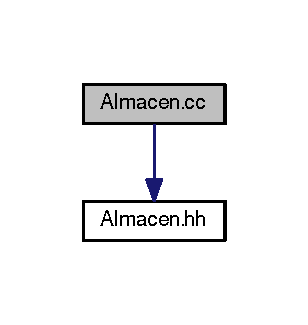
\includegraphics[width=148pt]{_almacen_8cc__incl}
\end{center}
\end{figure}

\hypertarget{_almacen_8hh}{}\section{Referencia del Archivo Almacen.\+hh}
\label{_almacen_8hh}\index{Almacen.\+hh@{Almacen.\+hh}}


Especificación de la clase \hyperlink{class_almacen}{Almacen}.  


\subsection*{Clases}
\begin{DoxyCompactItemize}
\item 
class \hyperlink{class_almacen}{Almacen}
\begin{DoxyCompactList}\small\item\em Representa la estructura del almacen. \end{DoxyCompactList}\end{DoxyCompactItemize}


\subsection{Descripción detallada}
Especificación de la clase \hyperlink{class_almacen}{Almacen}. 


\hypertarget{_cjt__productos_8cc}{}\section{Referencia del Archivo Cjt\+\_\+productos.\+cc}
\label{_cjt__productos_8cc}\index{Cjt\+\_\+productos.\+cc@{Cjt\+\_\+productos.\+cc}}


Código de la clase \hyperlink{class_cjt__productos}{Cjt\+\_\+productos}.  


Dependencia gráfica adjunta para Cjt\+\_\+productos.\+cc\+:\nopagebreak
\begin{figure}[H]
\begin{center}
\leavevmode
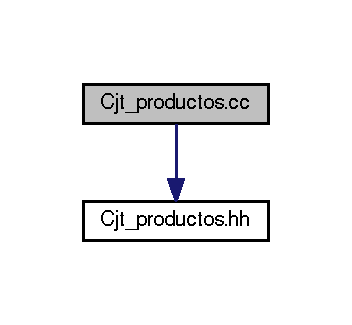
\includegraphics[width=169pt]{_cjt__productos_8cc__incl}
\end{center}
\end{figure}


\subsection{Descripción detallada}
Código de la clase \hyperlink{class_cjt__productos}{Cjt\+\_\+productos}. 


\hypertarget{_cjt__productos_8hh}{}\section{Referencia del Archivo Cjt\+\_\+productos.\+hh}
\label{_cjt__productos_8hh}\index{Cjt\+\_\+productos.\+hh@{Cjt\+\_\+productos.\+hh}}


Especificación de la clase \hyperlink{class_cjt__productos}{Cjt\+\_\+productos}.  


\subsection*{Clases}
\begin{DoxyCompactItemize}
\item 
class \hyperlink{class_cjt__productos}{Cjt\+\_\+productos}
\begin{DoxyCompactList}\small\item\em Representa el inventario del almacen con atributos identificador y unidades. \end{DoxyCompactList}\end{DoxyCompactItemize}


\subsection{Descripción detallada}
Especificación de la clase \hyperlink{class_cjt__productos}{Cjt\+\_\+productos}. 


\hypertarget{_cjt__salas_8cc}{}\section{Referencia del Archivo Cjt\+\_\+salas.\+cc}
\label{_cjt__salas_8cc}\index{Cjt\+\_\+salas.\+cc@{Cjt\+\_\+salas.\+cc}}


Código de la clase \hyperlink{class_cjt__salas}{Cjt\+\_\+salas}.  


Dependencia gráfica adjunta para Cjt\+\_\+salas.\+cc\+:\nopagebreak
\begin{figure}[H]
\begin{center}
\leavevmode
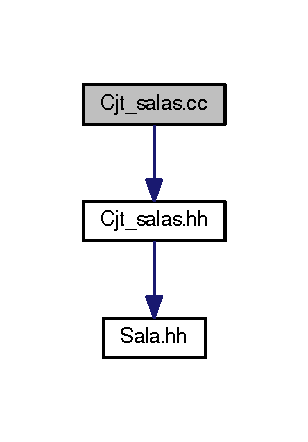
\includegraphics[width=148pt]{_cjt__salas_8cc__incl}
\end{center}
\end{figure}


\subsection{Descripción detallada}
Código de la clase \hyperlink{class_cjt__salas}{Cjt\+\_\+salas}. 


\hypertarget{_cjt__salas_8hh}{}\section{Referencia del Archivo Cjt\+\_\+salas.\+hh}
\label{_cjt__salas_8hh}\index{Cjt\+\_\+salas.\+hh@{Cjt\+\_\+salas.\+hh}}


Especificación de la clase \hyperlink{class_cjt__salas}{Cjt\+\_\+salas}.  


Dependencia gráfica adjunta para Cjt\+\_\+salas.\+hh\+:\nopagebreak
\begin{figure}[H]
\begin{center}
\leavevmode
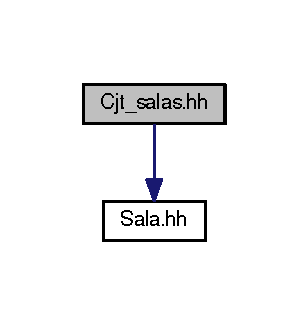
\includegraphics[width=148pt]{_cjt__salas_8hh__incl}
\end{center}
\end{figure}
\subsection*{Clases}
\begin{DoxyCompactItemize}
\item 
class \hyperlink{class_cjt__salas}{Cjt\+\_\+salas}
\begin{DoxyCompactList}\small\item\em Representa un conjunto de salas. \end{DoxyCompactList}\end{DoxyCompactItemize}


\subsection{Descripción detallada}
Especificación de la clase \hyperlink{class_cjt__salas}{Cjt\+\_\+salas}. 


\hypertarget{program_8cc}{}\section{Referència del Fitxer program.\+cc}
\label{program_8cc}\index{program.\+cc@{program.\+cc}}


Programa principal de la pràctica.  


Inclou el graf de dependències per a program.\+cc\+:\nopagebreak
\begin{figure}[H]
\begin{center}
\leavevmode
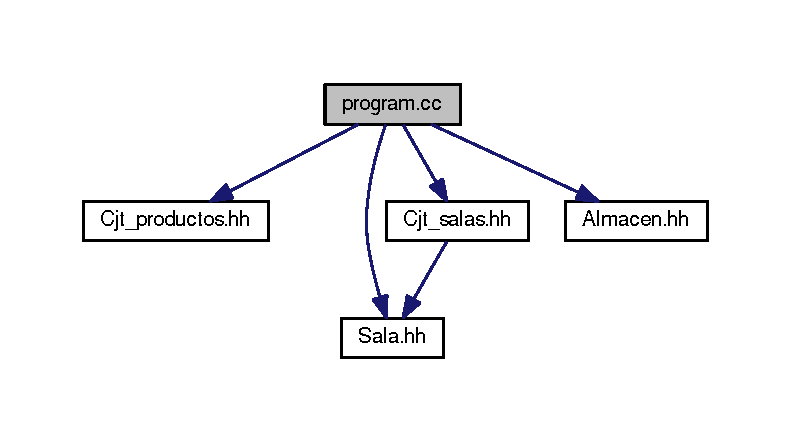
\includegraphics[width=256pt]{program_8cc__incl}
\end{center}
\end{figure}
\subsection*{Funcions}
\begin{DoxyCompactItemize}
\item 
int \hyperlink{program_8cc_ae66f6b31b5ad750f1fe042a706a4e3d4}{main} ()
\end{DoxyCompactItemize}


\subsection{Descripció Detallada}
Programa principal de la pràctica. 



\subsection{Documentació de les Funcions}
\mbox{\Hypertarget{program_8cc_ae66f6b31b5ad750f1fe042a706a4e3d4}\label{program_8cc_ae66f6b31b5ad750f1fe042a706a4e3d4}} 
\index{program.\+cc@{program.\+cc}!main@{main}}
\index{main@{main}!program.\+cc@{program.\+cc}}
\subsubsection{\texorpdfstring{main()}{main()}}
{\footnotesize\ttfamily int main (\begin{DoxyParamCaption}{ }\end{DoxyParamCaption})}



Definició a la línia 19 del fitxer program.\+cc.


\begin{DoxyCode}
19            \{
20     \textcolor{keywordtype}{int} k;
21     cin >> k;
22     \hyperlink{class_cjt___especies}{Cjt\_Especies} A;
23     \hyperlink{class_cjt___clusters}{Cjt\_Clusters} B;
24     \textcolor{keywordtype}{string} opcio;
25     \textcolor{keywordflow}{while} (cin >> opcio) \{
26         \textcolor{keywordflow}{if} (opcio == \textcolor{stringliteral}{"crea\_especie"}) \{
27             \textcolor{keywordtype}{string} id, g;
28             cin >> \textcolor{keywordtype}{id} >> g;
29             cout << \textcolor{stringliteral}{"# crea\_especie "} << \textcolor{keywordtype}{id} << \textcolor{stringliteral}{" "} << g << endl;
30             \textcolor{keywordflow}{if} (A.\hyperlink{class_cjt___especies_a2ce9d7a4968d46686109477f448857ea}{species\_exist}(\textcolor{keywordtype}{id})) \{
31                 cout << \textcolor{stringliteral}{"ERROR: La especie "}<< \textcolor{keywordtype}{id} << \textcolor{stringliteral}{" ya existe."} << endl;
32             \}
33             \textcolor{keywordflow}{else} \{
34                 \hyperlink{class_especie}{Especie} a(\textcolor{keywordtype}{id}, g, k);
35                 A.\hyperlink{class_cjt___especies_ab0aafd7fe0f24410a24aec9ff934bce0}{add\_species}(a);
36             \}
37             cout << endl;
38         \}
39         \textcolor{keywordflow}{else} \textcolor{keywordflow}{if} (opcio == \textcolor{stringliteral}{"obtener\_gen"}) \{
40             \textcolor{keywordtype}{string} id;
41             cin >> id;
42             cout << \textcolor{stringliteral}{"# obtener\_gen "} << \textcolor{keywordtype}{id} << endl;
43             \textcolor{keywordflow}{if} (A.\hyperlink{class_cjt___especies_a2ce9d7a4968d46686109477f448857ea}{species\_exist}(\textcolor{keywordtype}{id})) \{
44                 \hyperlink{class_especie}{Especie} a = A.\hyperlink{class_cjt___especies_a1e01bf8dfbde0983404efba05bd1b4b3}{find\_species}(\textcolor{keywordtype}{id});
45                 cout << a.\hyperlink{class_especie_a0781a594e45e036c0b59d161a7ebd8f3}{query\_gene}() << endl;
46             \}
47             \textcolor{keywordflow}{else} cout << \textcolor{stringliteral}{"ERROR: La especie "}<< \textcolor{keywordtype}{id} << \textcolor{stringliteral}{" no existe."} << endl;
48             cout << endl;
49         \}
50         \textcolor{keywordflow}{else} \textcolor{keywordflow}{if} (opcio == \textcolor{stringliteral}{"distancia"}) \{
51             \textcolor{keywordtype}{string} id1, id2;
52             cin >> id1 >> id2;
53             cout << \textcolor{stringliteral}{"# distancia "} << id1 << \textcolor{stringliteral}{" "} << id2 << endl;
54             \textcolor{keywordflow}{if} (not A.\hyperlink{class_cjt___especies_a2ce9d7a4968d46686109477f448857ea}{species\_exist}(id1) and not A.\hyperlink{class_cjt___especies_a2ce9d7a4968d46686109477f448857ea}{species\_exist}(id2)) cout << \textcolor{stringliteral}{"
      ERROR: La especie "} << id1 << \textcolor{stringliteral}{" y la especie "} << id2 << \textcolor{stringliteral}{" no existen."} << endl;
55             \textcolor{keywordflow}{else} \textcolor{keywordflow}{if} (not A.\hyperlink{class_cjt___especies_a2ce9d7a4968d46686109477f448857ea}{species\_exist}(id2)) cout << \textcolor{stringliteral}{"ERROR: La especie "} << id2 << \textcolor{stringliteral}{" no
       existe."} << endl;
56             \textcolor{keywordflow}{else} \textcolor{keywordflow}{if} (not A.\hyperlink{class_cjt___especies_a2ce9d7a4968d46686109477f448857ea}{species\_exist}(id1)) cout << \textcolor{stringliteral}{"ERROR: La especie "} << id1 << \textcolor{stringliteral}{" no
       existe."} << endl;
57             \textcolor{keywordflow}{else} cout << A.\hyperlink{class_cjt___especies_abf55093b325fd101ef73aa18dd1cf823}{species\_distance}(id1, id2) << endl;
58             cout << endl;
59 
60         \} 
61         \textcolor{keywordflow}{else} \textcolor{keywordflow}{if} (opcio == \textcolor{stringliteral}{"elimina\_especie"}) \{
62             \textcolor{keywordtype}{string} id;
63             cin >> id;
64             cout << \textcolor{stringliteral}{"# elimina\_especie "} << \textcolor{keywordtype}{id} << endl;
65             \textcolor{keywordflow}{if} (A.\hyperlink{class_cjt___especies_a2ce9d7a4968d46686109477f448857ea}{species\_exist}(\textcolor{keywordtype}{id})) \{
66                 A.\hyperlink{class_cjt___especies_ad72a47e0a785ac34f4908b54dd413d32}{erase\_species}(\textcolor{keywordtype}{id});
67             \} \textcolor{keywordflow}{else} cout << \textcolor{stringliteral}{"ERROR: La especie "} << \textcolor{keywordtype}{id} << \textcolor{stringliteral}{" no existe."} << endl;
68 
69             cout << endl;
70         \}
71         \textcolor{keywordflow}{else} \textcolor{keywordflow}{if} (opcio == \textcolor{stringliteral}{"existe\_especie"}) \{
72             \textcolor{keywordtype}{string} id;
73             cin >> id;
74             cout << \textcolor{stringliteral}{"# existe\_especie "} << \textcolor{keywordtype}{id} << endl;
75             \textcolor{keywordflow}{if} (A.\hyperlink{class_cjt___especies_a2ce9d7a4968d46686109477f448857ea}{species\_exist}(\textcolor{keywordtype}{id})) cout << \textcolor{stringliteral}{"SI"} << endl;
76             \textcolor{keywordflow}{else} cout << \textcolor{stringliteral}{"NO"} << endl;
77             cout << endl;
78         \} 
79         \textcolor{keywordflow}{else} \textcolor{keywordflow}{if} (opcio == \textcolor{stringliteral}{"lee\_cjt\_especies"}) \{
80             \textcolor{keywordtype}{int} n;
81             cin >> n;
82             A.\hyperlink{class_cjt___especies_a273156c50e67be8815bdd1c31cc1661a}{read\_species}(n, k);
83             cout << \textcolor{stringliteral}{"# lee\_cjt\_especies"} << endl;
84             cout << endl;
85             
86         \}
87         \textcolor{keywordflow}{else} \textcolor{keywordflow}{if} (opcio == \textcolor{stringliteral}{"imprime\_cjt\_especies"}) \{ \textcolor{comment}{//falta buidar}
88             cout << \textcolor{stringliteral}{"# imprime\_cjt\_especies"} << endl;
89             A.\hyperlink{class_cjt___especies_a362d2295d52e2a4cb3618bda7ad3f65b}{print\_species}();
90             cout << endl;
91         \}
92         \textcolor{keywordflow}{else} \textcolor{keywordflow}{if} (opcio == \textcolor{stringliteral}{"tabla\_distancias"}) \{
93             cout << \textcolor{stringliteral}{"# tabla\_distancias"} << endl;
94             A.\hyperlink{class_cjt___especies_ab6ebf81bf6ad734a970c3677fd4e5250}{print\_table\_species}();
95             cout << endl;
96         \}
97         \textcolor{keywordflow}{else} \textcolor{keywordflow}{if} (opcio == \textcolor{stringliteral}{"inicializa\_clusters"}) \{
98             cout << \textcolor{stringliteral}{"# inicializa\_clusters"} << endl;
99             B.\hyperlink{class_cjt___clusters_a35d2c4c28bee51017f4ac9049a0fe6e9}{initialize\_clusters}(A);
100             B.\hyperlink{class_cjt___clusters_acc4dd33e82c36c394acd44e60f77da22}{print\_table\_clusters}();
101             cout << endl;
102         \}
103 
104         \textcolor{keywordflow}{else} \textcolor{keywordflow}{if} (opcio == \textcolor{stringliteral}{"ejecuta\_paso\_wpgma"}) \{
105             cout << \textcolor{stringliteral}{"# ejecuta\_paso\_wpgma"} << endl;
106             \textcolor{keywordflow}{if} (B.\hyperlink{class_cjt___clusters_a1ecfc9a82c3a0dff467769880c355efd}{clusters\_set\_size}() > 1) \{
107                 B.\hyperlink{class_cjt___clusters_ac2bf2811c291533e3516ad4de8240d36}{wpgma\_algorithm}();
108                 B.\hyperlink{class_cjt___clusters_acc4dd33e82c36c394acd44e60f77da22}{print\_table\_clusters}();
109             \} \textcolor{keywordflow}{else} cout << \textcolor{stringliteral}{"ERROR: num\_clusters <= 1"} << endl;
110             cout << endl;
111         \}
112         \textcolor{keywordflow}{else} \textcolor{keywordflow}{if} (opcio == \textcolor{stringliteral}{"imprime\_cluster"}) \{
113             \textcolor{keywordtype}{string} id;
114             cin >> id;
115             cout << \textcolor{stringliteral}{"# imprime\_cluster "} << \textcolor{keywordtype}{id} << endl;
116             \textcolor{keywordflow}{if} (B.\hyperlink{class_cjt___clusters_aaa57cbd8d86567b4403ac9adb34a87f5}{cluster\_exist}(\textcolor{keywordtype}{id})) \{
117                 \hyperlink{class_cluster}{Cluster} aux = B.\hyperlink{class_cjt___clusters_a4ab91d8e8222f35b4c9592c5ab2b4bf3}{find\_cluster}(\textcolor{keywordtype}{id});
118                 B.\hyperlink{class_cjt___clusters_aa9a896c44d86f130747f1e6821a4dddd}{print\_cluster}(aux);
119                 cout << endl;
120             \} \textcolor{keywordflow}{else} cout << \textcolor{stringliteral}{"ERROR: El cluster "} << \textcolor{keywordtype}{id} << \textcolor{stringliteral}{" no existe."} << endl;
121             cout << endl;
122         \}
123         \textcolor{keywordflow}{else} \textcolor{keywordflow}{if} (opcio == \textcolor{stringliteral}{"imprime\_arbol\_filogenetico"}) \{
124             cout << \textcolor{stringliteral}{"# imprime\_arbol\_filogenetico"} << endl;
125             B.\hyperlink{class_cjt___clusters_a35d2c4c28bee51017f4ac9049a0fe6e9}{initialize\_clusters}(A);
126             \textcolor{keywordflow}{if} (B.\hyperlink{class_cjt___clusters_a1ecfc9a82c3a0dff467769880c355efd}{clusters\_set\_size}() < 1) cout << \textcolor{stringliteral}{"ERROR: El conjunto de clusters es
       vacio."} << endl;
127             \textcolor{keywordflow}{else} \{
128                 \textcolor{keywordflow}{while} (B.\hyperlink{class_cjt___clusters_a1ecfc9a82c3a0dff467769880c355efd}{clusters\_set\_size}() > 1) \{
129                     B.\hyperlink{class_cjt___clusters_ac2bf2811c291533e3516ad4de8240d36}{wpgma\_algorithm}();
130                 \}
131                 \hyperlink{class_cluster}{Cluster} aux = B.\hyperlink{class_cjt___clusters_a48cb7ca0417ba1de9593a00f98d91880}{query\_final\_cluster}();
132                 B.\hyperlink{class_cjt___clusters_aa9a896c44d86f130747f1e6821a4dddd}{print\_cluster}(aux);
133                 
134 
135                 cout << endl;
136             \}
137             cout << endl;
138         \}
139         \textcolor{keywordflow}{else} \textcolor{keywordflow}{if} (opcio == \textcolor{stringliteral}{"fin"}) \{
140             \textcolor{keywordflow}{break};
141         \}
142     \}
143 
144 
145 \}
\end{DoxyCode}

\hypertarget{_sala_8cc}{}\section{Referencia del Archivo Sala.\+cc}
\label{_sala_8cc}\index{Sala.\+cc@{Sala.\+cc}}


Código de la clase \hyperlink{class_sala}{Sala}.  


Dependencia gráfica adjunta para Sala.\+cc\+:\nopagebreak
\begin{figure}[H]
\begin{center}
\leavevmode
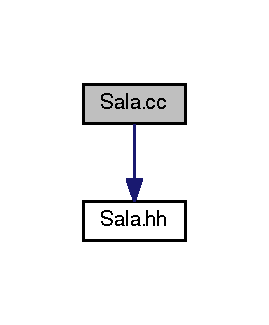
\includegraphics[width=129pt]{_sala_8cc__incl}
\end{center}
\end{figure}


\subsection{Descripción detallada}
Código de la clase \hyperlink{class_sala}{Sala}. 


\hypertarget{_sala_8hh}{}\section{Referencia del Archivo Sala.\+hh}
\label{_sala_8hh}\index{Sala.\+hh@{Sala.\+hh}}


Especificación de la clase \hyperlink{class_sala}{Sala}.  


\subsection*{Clases}
\begin{DoxyCompactItemize}
\item 
class \hyperlink{class_sala}{Sala}
\begin{DoxyCompactList}\small\item\em Representa una sala del almacen. \end{DoxyCompactList}\end{DoxyCompactItemize}


\subsection{Descripción detallada}
Especificación de la clase \hyperlink{class_sala}{Sala}. 


%--- End generated contents ---

% Index
\backmatter
\newpage
\phantomsection
\clearemptydoublepage
\addcontentsline{toc}{chapter}{Índice}
\printindex

\end{document}
